\chapter{Description des données}
\vspace{-1.5em}
\chaptertoc
\vspace{-2.5em}
\vspace{-0.5em}
\section{Introduction}
\vspace{-1em}
L’industrie aéronautique génère de grandes quantités de données. Ce chapitre présente d’abord les sources et la structure des jeux de données utilisés, puis les résultats de l’analyse exploratoire (\ac{AED}) permettant d’identifier les tendances et anomalies. Il détaille ensuite les étapes de prétraitement nécessaires pour préparer les données à l’analyse.

\vspace{-1.5em}
\section{Source des données}
\vspace{-0.7em}
L’ensemble de données utilisé dans cette étude provient des processus opérationnels liés à la planification des vols saisonniers dans les aéroports marocains. Plus précisément, les données sont issues des horaires de vol soumis par les compagnies aériennes, validés par le \ac{MSC}, puis traités par \ac{CPV}. Ces informations sont initialement échangées sous forme de fichiers Excel, ajustées manuellement, puis intégrées dans le système \ac{SOAM} pour l’allocation des ressources aéroportuaires.  

\begin{figure}[H]
	\centering
	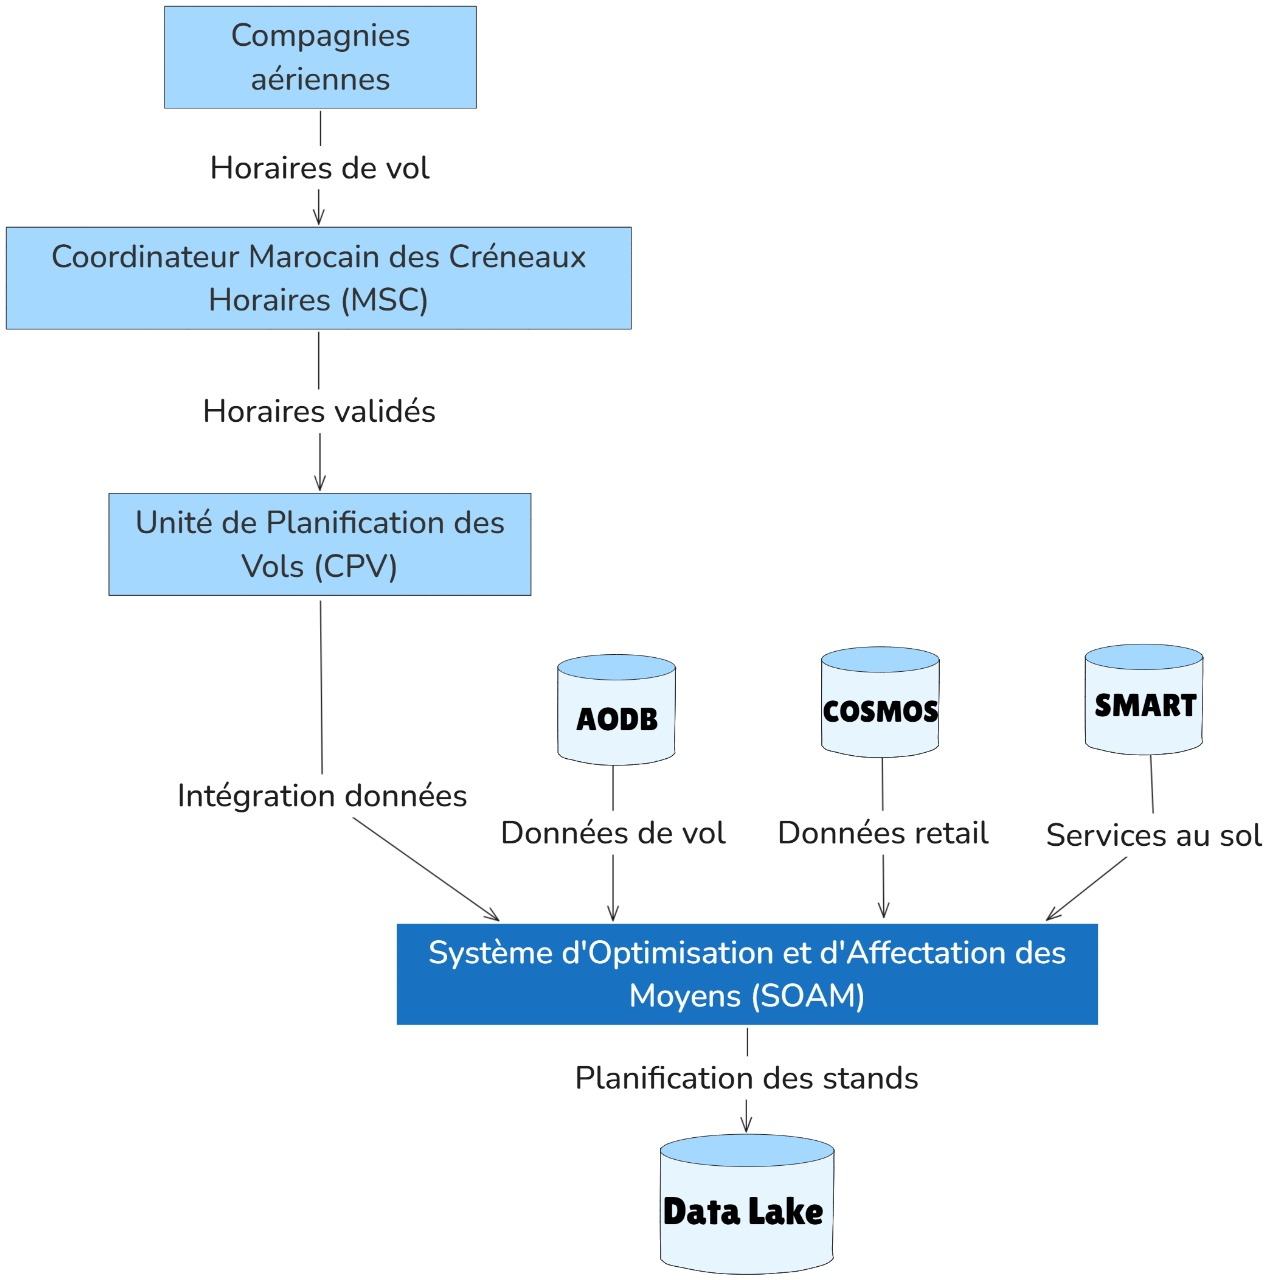
\includegraphics[width=0.6\linewidth]{assets/dataset/flux Données.jpg}
	\caption{Flux de données}
	\label{fig:flux_donnees}
\end{figure}


Le schéma \ref{fig:flux_donnees} illustre le flux de données depuis les compagnies aériennes jusqu'à l'intégration dans le \ac{SOAM}.
Les données exploitées dans cette étude couvrent un large spectre d’informations relatives à la planification des stands, comprenant des éléments statiques et dynamiques.

\subsection*{Synthèse des Sources de Données}
Les données exploitées proviennent de différentes sources internes et externes.

\noindent\textbf{Métadonnées des flux}~: Données extraites des tables Oracle, mises à jour toutes les 2h (quasi temps réel), avec un chargement initial complet puis des mises à jour incrémentales. Formats : JSON/Excel. Protocole à définir selon les systèmes.

\vspace{0.8em}
\noindent\textbf{Catégories de données opérationnelles} :
\begin{itemize}
	\item \textbf{Vols} (\acs{AODB})~: arrivées, départs, retards, statuts, mouvements, horaires ajustés, type de vol.
	\item \textbf{Avions et stands}~: types d’appareils, occupation des stands, durée escale, night stops, capacités, référentiels.
	\item \textbf{Infrastructure et sécurité}~: proximité équipements (passerelles, carburant), séparations de sécurité, zones sensibles, stands maintenance.
	\item \textbf{Données complémentaires}~: météo, consommation énergétique, activité commerciale (\textsc{COSMOS}/SMART).
\end{itemize}


\subsection*{Répartition de Source de données}
La répartition des sources de données, illustrée dans la Figure \ref{fig:enter-label}, montre une prédominance marquée de l'\ac{AODB}, qui représente à elle seule 70 \% des sources utilisées. Les aéroports contribuent pour 15 \%, tandis que les autres sources, notamment COSMOS/SMART, se partagent les 15 \% restants. Cette distribution met en évidence la centralité de l'\ac{AODB} dans le système.
\begin{figure}[H]
	\centering
	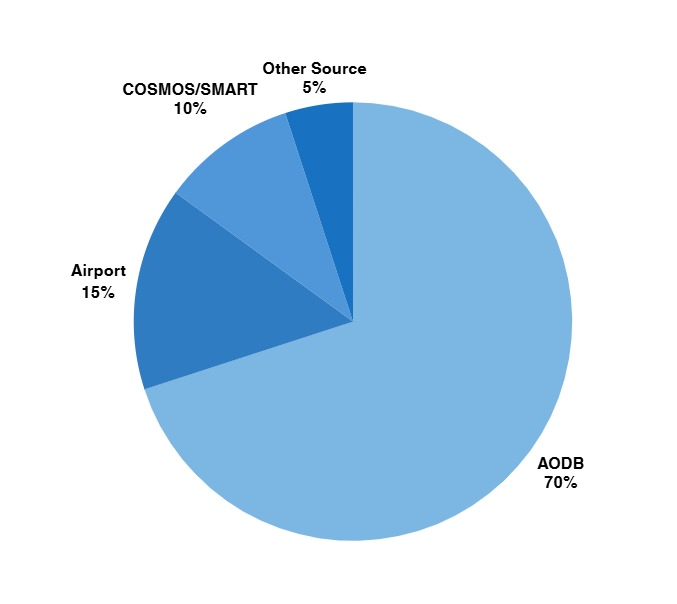
\includegraphics[width=0.5\linewidth]{assets/dataset/Distribution.jpg}
	\caption{Répartition de Catégories de données}
	\label{fig:enter-label}
\end{figure}

Toutes ces sources de données ont été exploitées dans le but de constituer un jeu de données unifié. Après l'étape de collecte, l’ensemble des informations a été consolidé en deux fichiers CSV finaux, utilisés comme base pour nos analyses.



\section{Description des données}
Dans cette étape, nous commençons par explorer la structure et le contenu de l'ensemble de données aéroportuaires pour comprendre ses composantes clés et les relations entre elles. Alors notre étude s'appuie sur deux jeux de données principaux :  

\_{Un dataset dédié aux départs de vols \textbf{(4945 observations, 485 variables)}}.  

\_{Un second relatif aux arrivées de vols \textbf{(5018 observations, 417 variables)}, partageant une structure similaire mais présentant des variations contextuelles dans l'agencement des lignes et de certaines colonnes.}

En raison de la complexité inhérente à ces données multidimensionnelles, une catégorisation thématique a été mise en place pour en faciliter l'analyse et l'interprétation. Cette segmentation, représentée par un organigramme dans la Figure~\ref{fig:dataset} qui regroupe les variables en catégories fonctionnelles:

\begin{itemize}
	\item \textbf{Vols et compagnies aériennes} : Cette catégorie regroupe les informations liées aux vols, aux compagnies aériennes, aux villes, aux avions, ainsi qu’aux aéroports concernés.
	\item \textbf{Infrastructures aéroportuaires} : Elle inclut des détails sur les terminaux, les stands, les portes d’embarquement et autres éléments liés aux installations de l’aéroport.
	\item \textbf{Temps et dates} : Cette catégorie regroupe les informations temporelles comme les horaires de départ et d’arrivée, planifiés et réels, les fuseaux horaires et les périodes d’exploitation.
	\item \textbf{Bagages et passagers} : Ce volet couvre les systèmes de gestion des bagages, les délais de traitement et les infrastructures associées.
	\item \textbf{Retards et irrégularités} : Contient des informations sur la durée des retards ainsi que les perturbations impactant les vols.
	\item \textbf{Opérations au sol} : Données sur les procédures avant départ ou après arrivée.
	\item \textbf{Divers} : Regroupe les variables hors des catégories précédentes.
\end{itemize}
\begin{figure}[H]
	\centering
	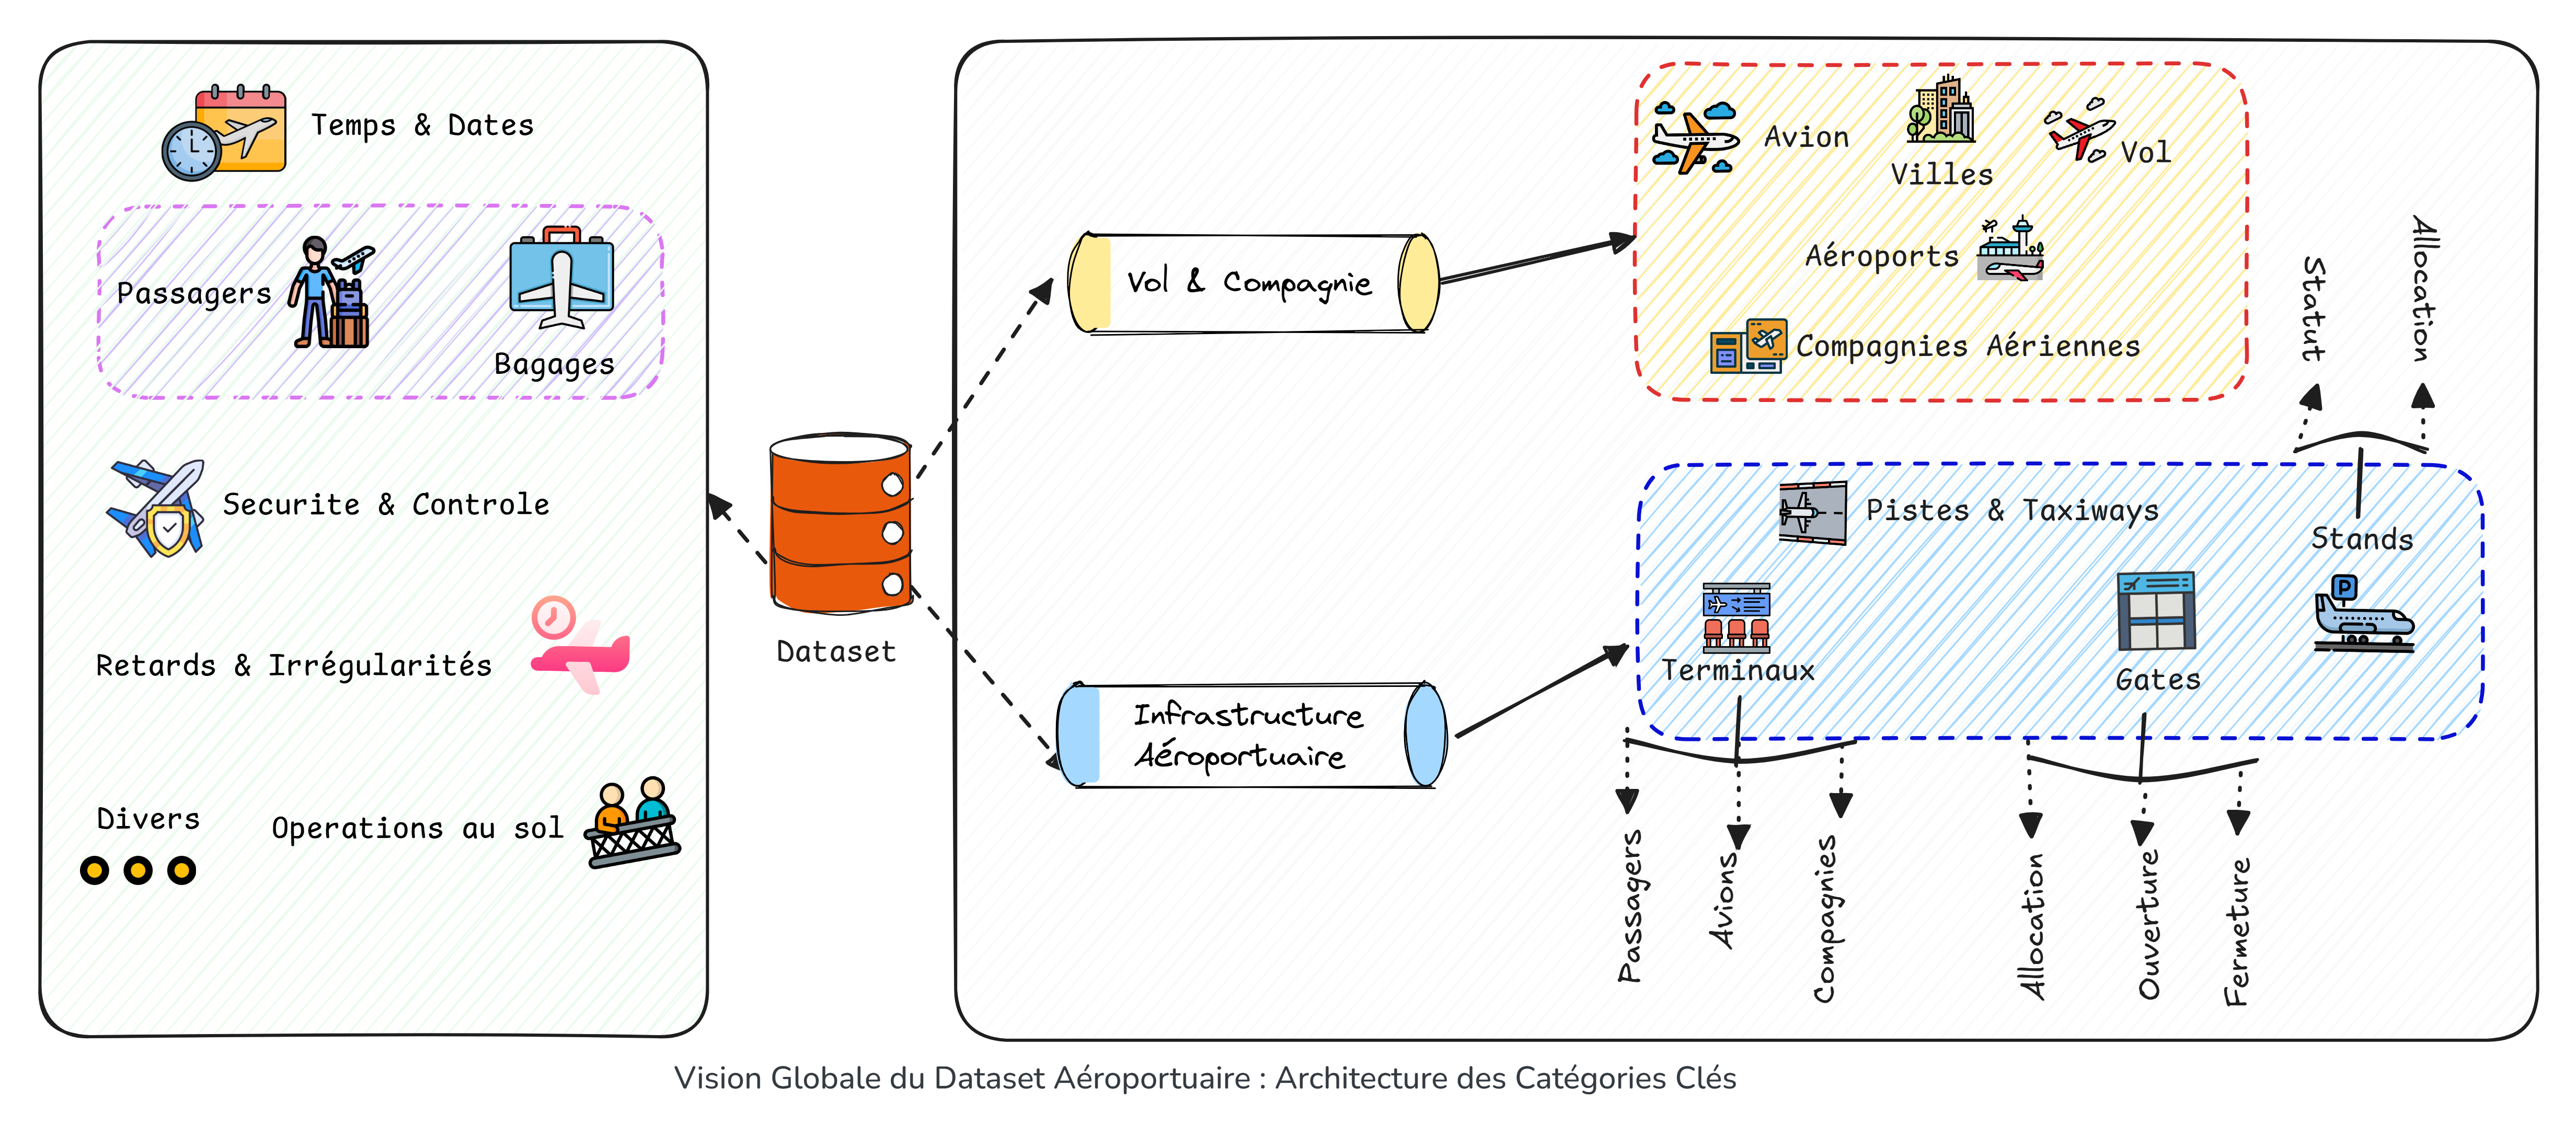
\includegraphics[width=0.9\linewidth]{assets/dataset/dataset.png}
	\caption{Illustration du dataset}
	\label{fig:dataset}
\end{figure}

Cette organisation favorise une analyse plus efficace du dataset en regroupant les informations selon leur nature et leur impact sur les opérations aéroportuaires. Elle facilite également l'interprétation des résultats et met en lumière les relations entre les différentes variables du dataset.

\subsection*{Vue d’ensemble des données opérationnelles}
Le tableau \ref{tab:synthese_operationnelle} ci-dessous résume les principales caractéristiques du jeu de données utilisé dans cette étude. Il s'agit de données opérationnelles collectées sur une période de deux mois (novembre et décembre 2024).

\begin{table}[H]
	\centering
	\renewcommand{\arraystretch}{0.9} % réduit l'espacement vertical
	\caption{Synthèse des données opérationnelles aéroportuaires}
	\begin{tabularx}{\textwidth}{@{}>{\bfseries}l X@{}}
		\toprule
		\textbf{Paramètre} & \textbf{Caractéristiques} \\
		\midrule
		Période du trafic          & 2 mois (Novembre \& Décembre 2024) \\
		Volume de trafic           & 9\,963 vols \\
		Variables – Dataset départ & 485 \\
		Variables – Dataset arrivée& 417 \\
		Opérateurs aériens         & 46 compagnies aériennes \\
		Catégorie opérationnelle   & Transport de passagers \\
		Nombre de stands           & 65 stands de stationnement \\
		Type de vols               & International / Domestique \\
		Vols Schengen              & SCH ou non \\
		Type d'avion               & A320, B737, B787, A330, A380 \\
		Classification des retards & Aucun, Faible, Moyen, Élevé, Majeur \\
		\bottomrule
	\end{tabularx}

	\label{tab:synthese_operationnelle}
\end{table}

\noindent
Il est important de noter que les données disponibles couvrent uniquement une période de deux mois. En réalité, l'aéroport traite un volume bien plus important : un plus grand nombre de compagnies aériennes, une diversité accrue de types d’avions, ainsi que 83 stands utilisés, incluant ceux destinés aux vols réguliers, au fret (cargo) et à la maintenance (hangars).




\section{Analyse et Visualisation des Données}

Pour acquérir une compréhension approfondie de l'ensemble de données aéroportuaires et en tirer des insights significatifs, un cadre d’analyse structuré a été établi. Celui-ci commence par le prétraitement des données brutes — incluant les vols, les stands, les portes d'embarquement, les terminaux et les retards — à travers des étapes de nettoyage et de transformation.

L’ensemble de données est ensuite exploré selon trois axes analytiques principaux :
\begin{itemize}
	\item \textbf{Analyse des vols} : étude des caractéristiques des vols, des horaires, des types d’appareils, ainsi que des compagnies aériennes les plus actives.
	\item \textbf{Analyse des stands} : évaluation du nombre total de stands, des compagnies utilisatrices, et de la durée moyenne de stationnement.
	\item \textbf{Analyse des retards} : analyse des vols retardés, des durées maximales de retard et des compagnies les plus fréquemment concernées.
\end{itemize}

Les résultats obtenus permettent d’identifier des modèles clés tels que les taux d’occupation, les flux horaires et les tendances de trafic. Cette compréhension globale facilite la production de visualisations claires et éclairées la planification optimale des ressources aéroportuaires.

\subsection{Analyse des vols}

Dans cette partie, une analyse des caractéristiques générales des vols du dataset a été réalisée, visant à identifier les tendances liées aux horaires, aux compagnies aériennes et aux types d’avions.

\begin{figure}[H]
	\centering
	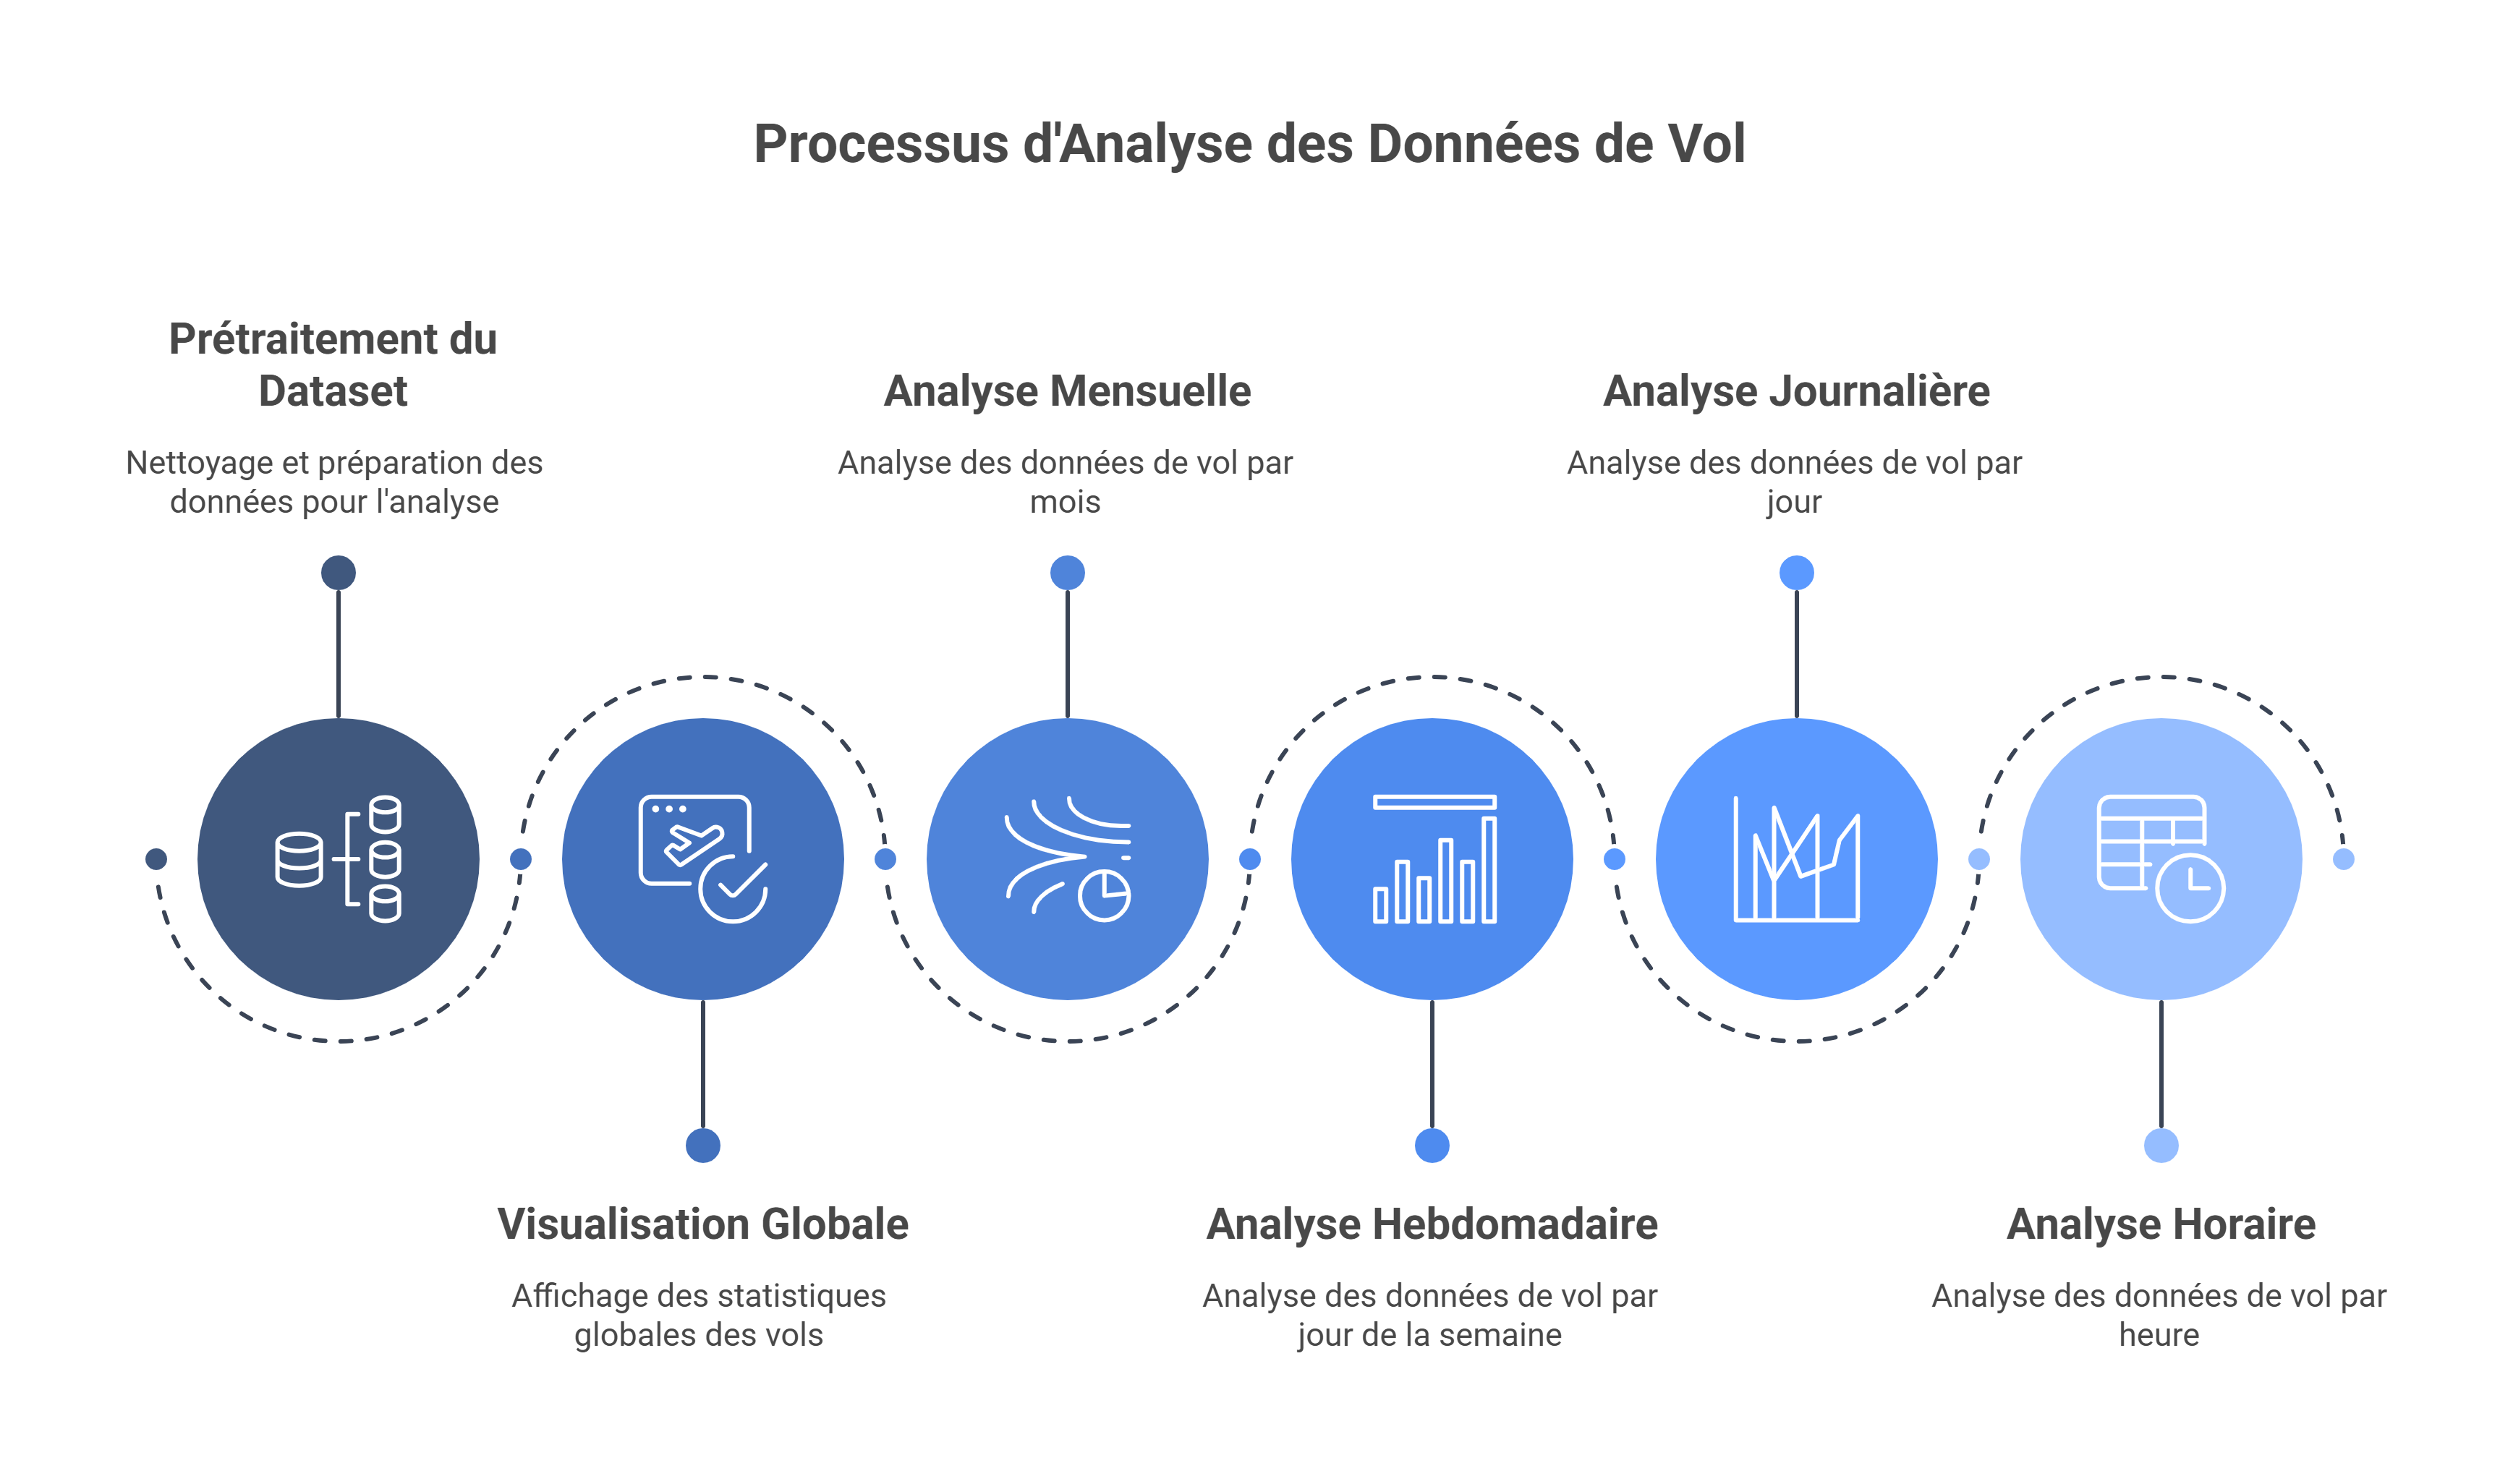
\includegraphics[width=0.8\textwidth]{assets/dataset/vol1.png}
	\caption{Flux du processus d'analyse des vols.}
	\label{fig:flight_analysis_flow}
\end{figure}

Afin d’assurer un processus méthodique, l’analyse suit la structure décrite ci-dessous :

Tout d’abord, une phase de prétraitement est effectuée pour préparer les données à l’analyse.  
Ensuite, une visualisation globale est réalisée afin d’avoir une vue d’ensemble du jeu de données.  
L’analyse est ensuite affinée selon trois niveaux temporels: \begin{itemize}
	\item Une analyse mensuelle pour identifier les tendances générales,
	\item Une analyse hebdomadaire pour un suivi plus précis,
	\item Une analyse journalière pour détecter les variations quotidiennes.
\end{itemize}

Enfin, une analyse horaire est menée afin de mieux comprendre la dynamique des vols selon les différentes tranches horaires de la journée.

Cette approche progressive permet d’avoir une vision détaillée du comportement des vols.  
\subsubsection{prétraitement de données}
Avant de procéder à l’analyse principale, une phase de prétraitement essentielle
est réalisée afin de préparer le jeu de données. Cette étape garantit que les données
sont propres, pertinentes et correctement structurées pour les opérations à venir. Le
prétraitement suit le schéma illustré ci-dessous.
\begin{figure}[H]
	\centering
	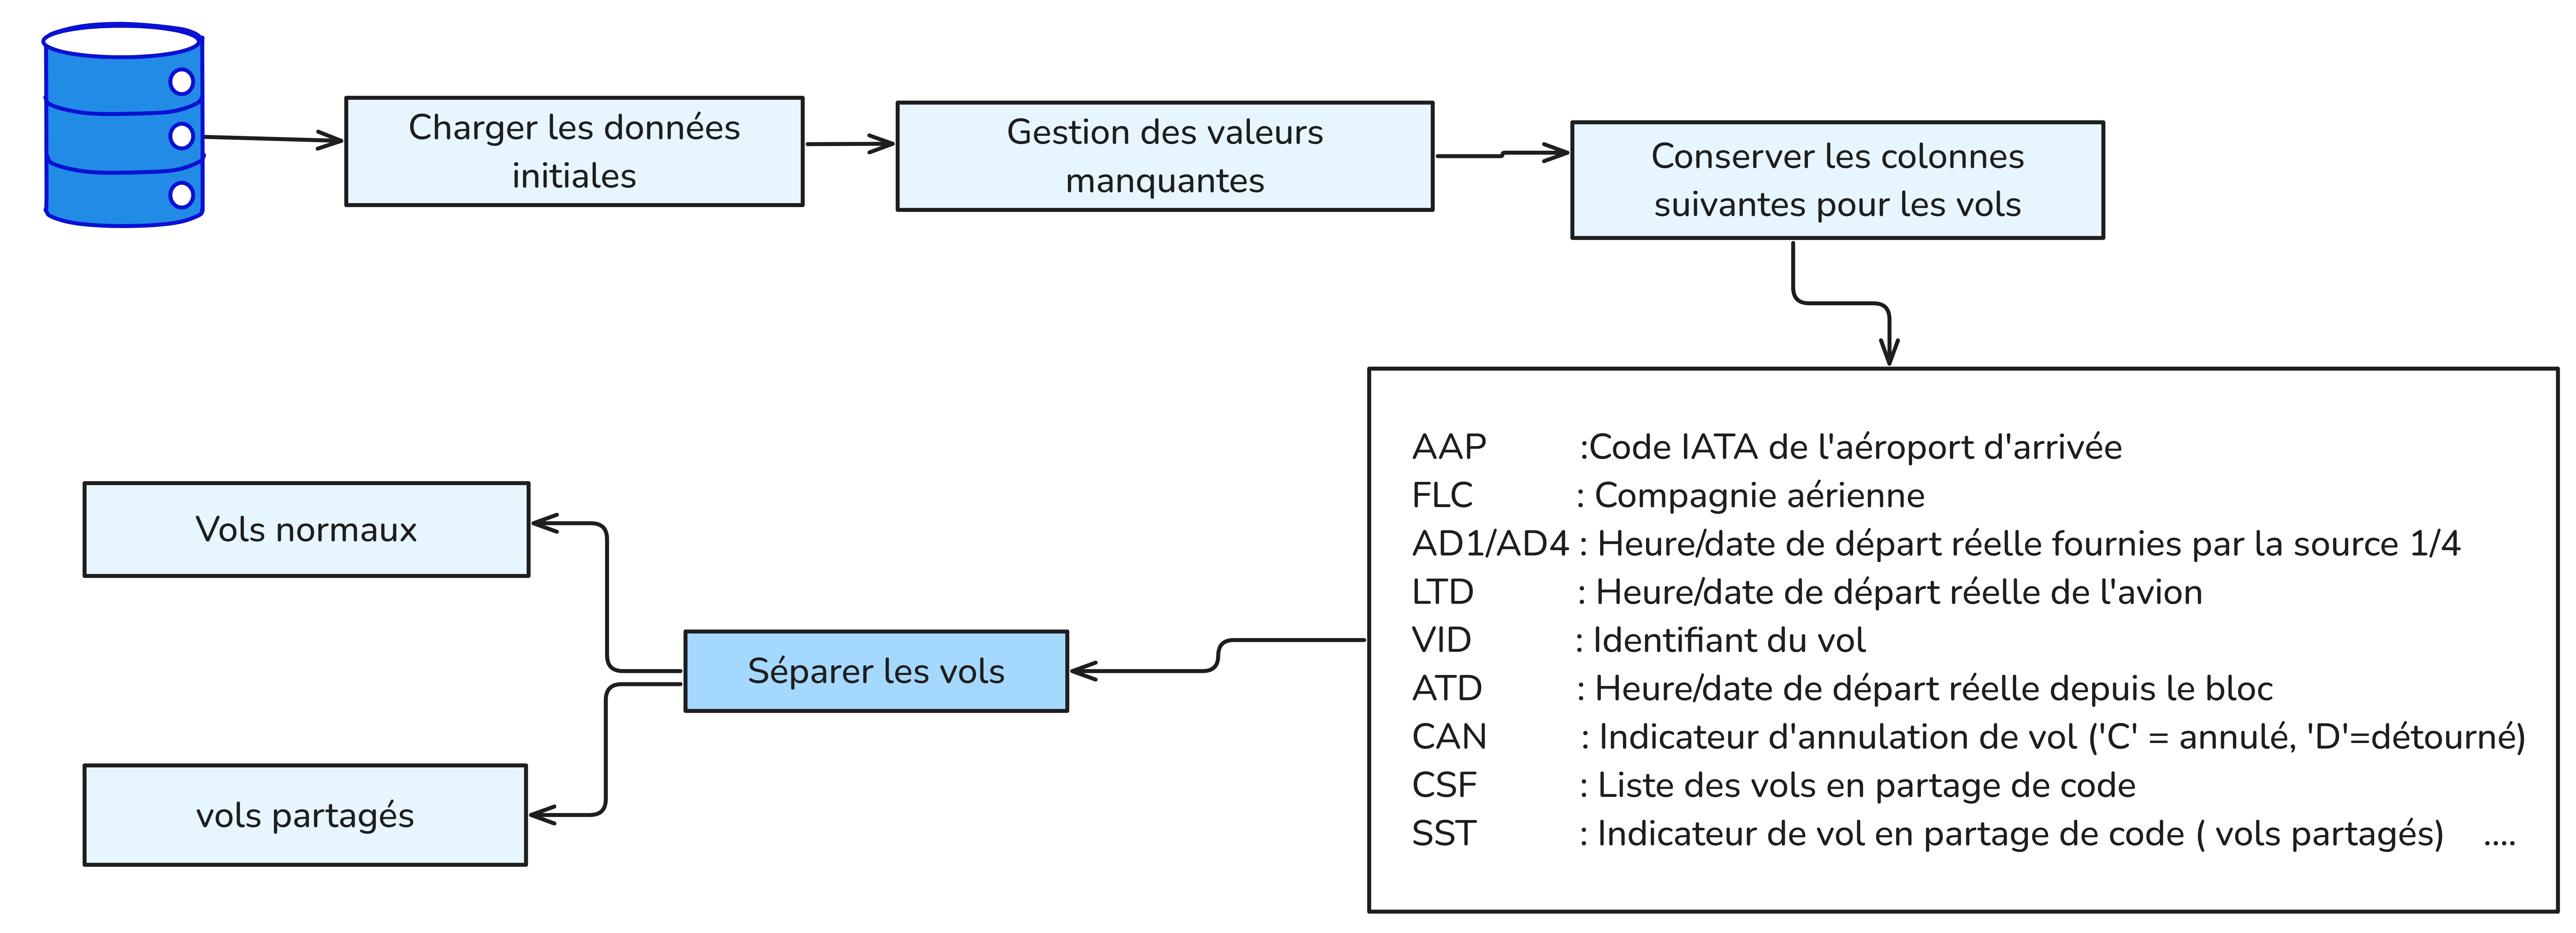
\includegraphics[width=0.9\textwidth]{assets/dataset/preprocessing.png} % adapt the filename
	\caption{Organigramme du prétraitement du jeu de données.}
	\label{fig:preprocessing_flowchart}
\end{figure}

Le prétraitement comprend les étapes suivantes :

\begin{itemize}
	\item\textbf{Chargement du jeu de données initial}:
	Le jeu de données original contenant les informations sur les vols est importé dans le système.
	
	\item \textbf{Traitement des valeurs manquantes} : Les entrées manquantes ou incomplètes sont gérées afin d’assurer la cohérence du jeu de données, notamment à l’aide de techniques d’imputation (comme la substitution par la moyenne, la médiane ou des valeurs prédites).
	
	
	\item \textbf{ Sélection des colonnes pertinentes}: Seules les colonnes essentielles à l’analyse des vols sont conservées. Celles-ci incluent les identifiants des vols, les heures de départ et d’arrivée, les compagnies aériennes, les indicateurs d’annulation, et les marqueurs de vols partagés.
	
	\item \textbf{Séparation des vols}: Le jeu de données est divisé en deux catégories :
	\begin{itemize}
		\item \textit{Vols normaux}: Vols standards, indépendants.
		\item \textit{Vols en partage de code}: Vols opérés dans le cadre d’un accord de partage de code entre plusieurs compagnies.
	\end{itemize}
\end{itemize}

Ce prétraitement permet d’assurer que les données utilisées pour l’analyse sont
à la fois propres et spécifiquement adaptées aux objectifs de l’étude. 

\subsubsection{Analyse Globale du Jeu de Données}

Pour initier notre étude, une analyse globale du jeu de données a été réalisée à travers diverses visualisations afin de mieux comprendre la structure sous-jacente des données.

Dans un premier temps, nous avons examiné la tendance globale du trafic aérien sur la période de deux mois étudiée. Nous avons observé un pic d’activité en novembre, indiquant une augmentation significative du nombre de vols par rapport au mois suivant.

Ensuite, nous avons analysé la répartition des vols par compagnie aérienne. Cette analyse a révélé que la compagnie \textbf{\ac{AT}} a opéré le plus grand nombre de vols, suivie par \textbf{3O} (Air Arabia) et \textbf{AF} (Air France).
\begin{figure}[H]
	\centering
	\begin{minipage}{0.25\textwidth}
		\centering
		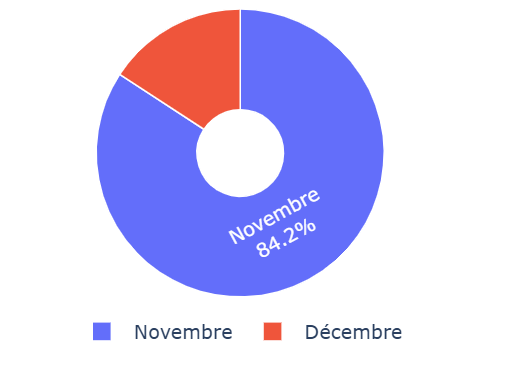
\includegraphics[width=\linewidth]{assets/dataset/repartitionpourcen.png}
		\small a) La tendance des vols globale entre novembre et décembre
	\end{minipage}
	\hfill
	\begin{minipage}{0.7\textwidth}
		\centering
		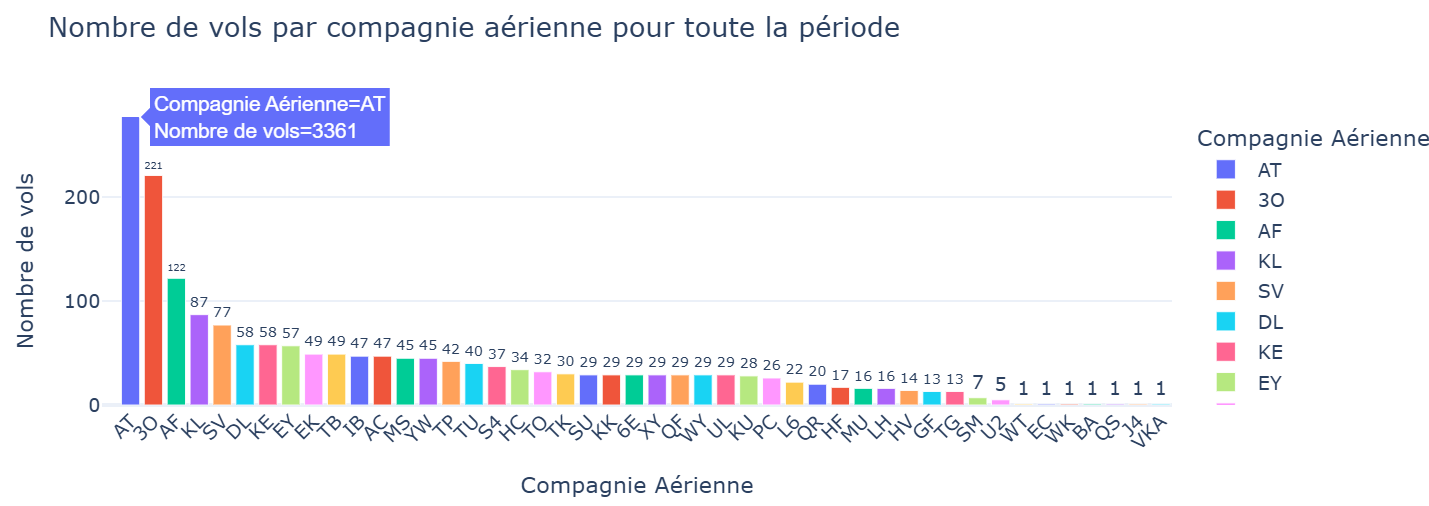
\includegraphics[width=\linewidth]{assets/dataset/nmbrvols.png}
		\small b) Répartition des vols par compagnie aérienne
	\end{minipage}
	
	\captionsetup{justification=centering}
	\caption{Les Vols en (novembre -décembre.) et répartition par compagnie.}
	\label{fig:analyse_trafic}
\end{figure}
\vspace{-0.5cm}
Le jeu de données distinguant deux types de vols: les \textbf{\textit{vols normaux}} et les \textbf{\textit{vols en partage de code}}. Nous avons approfondi l’analyse de leur répartition. Un vol en partage de code est défini comme un vol opéré par une compagnie aérienne mais commercialisé sous plusieurs numéros de vols par des compagnies partenaires,
éventuellement associées à différents codes des compagnies aériennes.
\newline
Notre analyse a montré que certaines compagnies n’opéraient que des vols en partage de code, sans présence opérationnelle directe. Par conséquent, ces compagnies ont été exclues du processus d’allocation des postes de stationnement. À l’inverse, l’attention a été portée sur les compagnies opérant leurs propres vols, qu’ils soient normaux ou en partage de code.  

La \textbf{Figure~\ref{fig:analyse_trafic}}  ainsi que La \textbf{Figure~\ref{fig:analyse_vols_partage}} 
ci-dessous illustre cette distinction.

\begin{figure}[H]
	\centering
	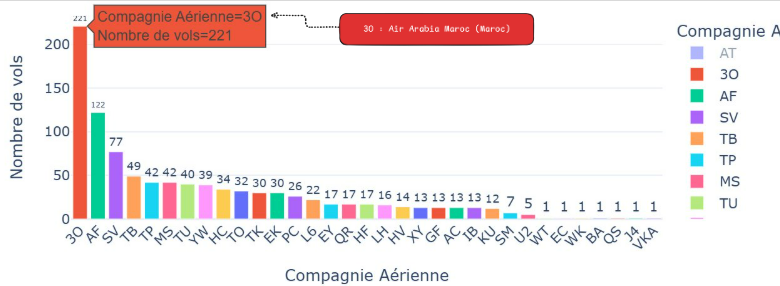
\includegraphics[width=0.95\textwidth]{assets/dataset/sansSF.png}
	\captionsetup{justification=centering}
	\caption{Vols par compagnie actives uniquement}
	\label{fig:analyse_vols_partage}
\end{figure}
 On y observe notamment que la compagnie \textbf{KL} (KLM Royal Dutch Airlines) est uniquement présente dans les vols en partage de code, ce qui indique qu’elle n'opère aucun vol avec ses propres aéronefs durant la période analysée.  
 
La \textbf{Figure~\ref{fig:vols_partages_compagnie}}  montre la répartition des vols partagés par compagnie .
\begin{figure}[H]
	\centering
	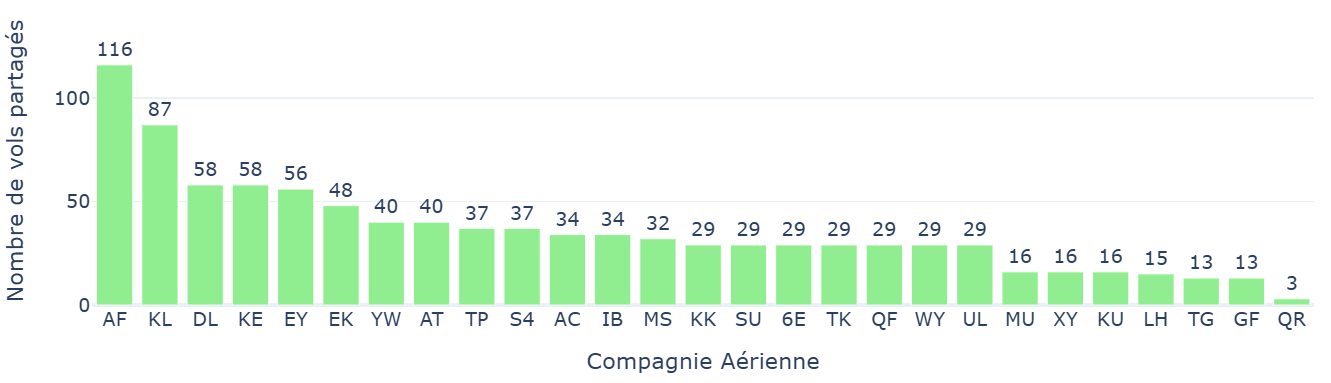
\includegraphics[width=1\textwidth]{assets/dataset/nbrvolsSF.png}
	\captionsetup{justification=centering}
	\caption{Vols partagés par compagnie}
	\label{fig:vols_partages_compagnie}
\end{figure}




Enfin, une attention particulière a été accordée aux taux d’annulation par compagnie aérienne. L’analyse de la proportion de vols annulés nous a permis de mieux comprendre la fiabilité de chaque compagnie et d’anticiper d’éventuelles perturbations dans les analyses ultérieures.

\subsubsection{Analyse Mensuelle, Hebdomadaire, Journalière et Horaire}

À la suite de l’analyse globale, nous avons procédé à une étude temporelle plus détaillée, en commençant par une décomposition mensuelle.

Étant donné que le mois de novembre a présenté le volume de vols le plus élevé, nous avons centré notre analyse sur ce mois. Nous avons ensuite ciblé les deux semaines présentant le pic d’activité au cours de novembre, afin d’obtenir une compréhension plus précise de la répartition du trafic.

La figure \ref{fig:repartition_vols_par_semaine} présente la répartition des vols par semaine pour le mois de Novembre
\begin{figure}[H]
	\centering
	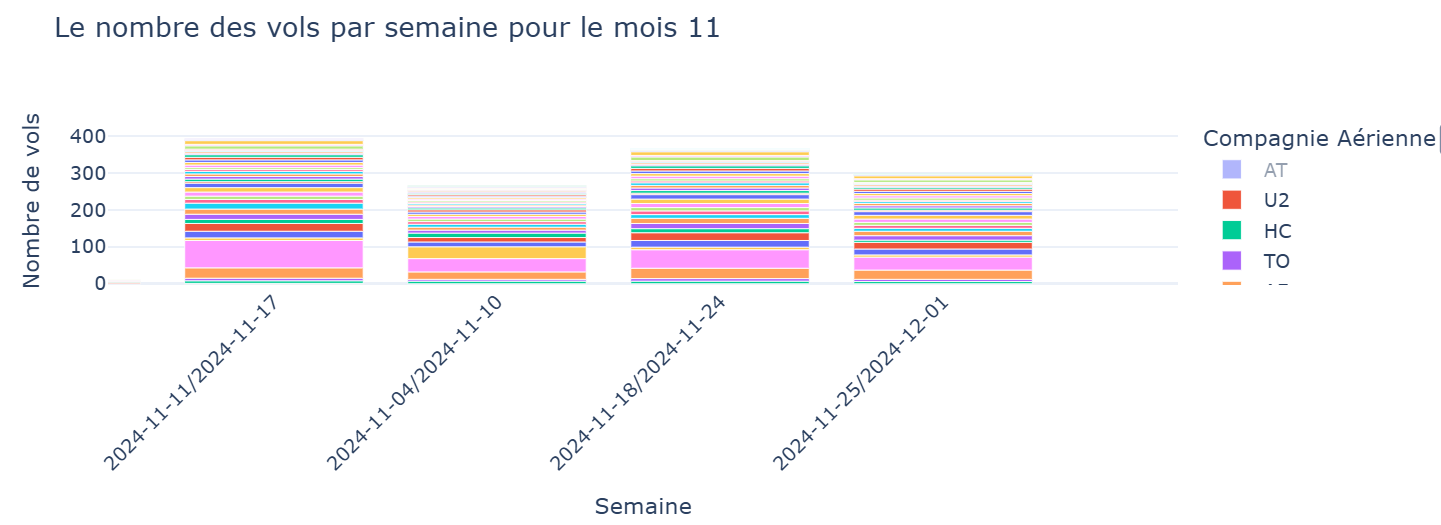
\includegraphics[width=1\textwidth]{assets/dataset/repartitionvolsparsemaine.png}
	\captionsetup{justification=centering}
	\caption{Répartition des vols par semaine}
	\label{fig:repartition_vols_par_semaine}
\end{figure}
Par la suite, nous avons affiné l’analyse en étudiant les tendances journalières et horaires. Cette approche de zoom progressif nous a permis d’identifier les jours les plus chargés ainsi que les heures de pointe, fournissant ainsi des informations critiques pour l’optimisation des opérations et l’allocation des postes de stationnement.
\begin{figure}[H]
	\centering
	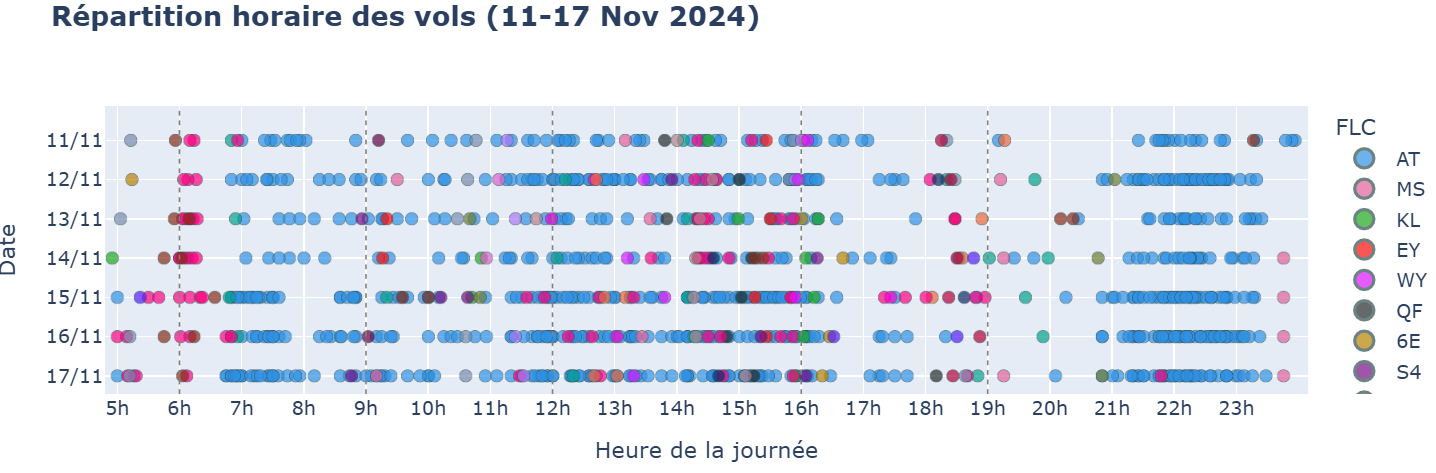
\includegraphics[width=1\textwidth]{assets/dataset/repartitionparheure.png}
	\captionsetup{justification=centering}
	\caption{Répartition des vols par heure durant la semaine la plus chargée}
	\label{fig:repartition_vols_par_heure}
\end{figure}
\vspace{-0.7em}
La figure montre une concentration du trafic entre \textbf{12h et 16h}, période durant laquelle le volume de vols atteint son pic.

\vspace{-0.7em}
\subsection{Analyse des stands}
De même, une analyse des caractéristiques générales des stands du dataset a été réalisée.
\subsubsection{Sélection des caractéristiques}

La première étape de l’analyse des stands a consisté en une sélection rigoureuse des caractéristiques pertinentes, comme illustré dans la figure~\ref{fig:stand-selection}. Plus précisément, nous avons retenu les colonnes directement liées à l’occupation des stands, à leur disponibilité, ainsi qu’à leur attribution au cours des périodes temporelles. Par la suite, une phase de prétraitement a été réalisée afin de traiter les valeurs manquantes, de standardiser les formats et d’assurer la cohérence des données. Ce travail préparatoire était essentiel pour permettre une analyse précise et fiable dans les étapes suivantes.


\begin{figure}[h]
	\centering
	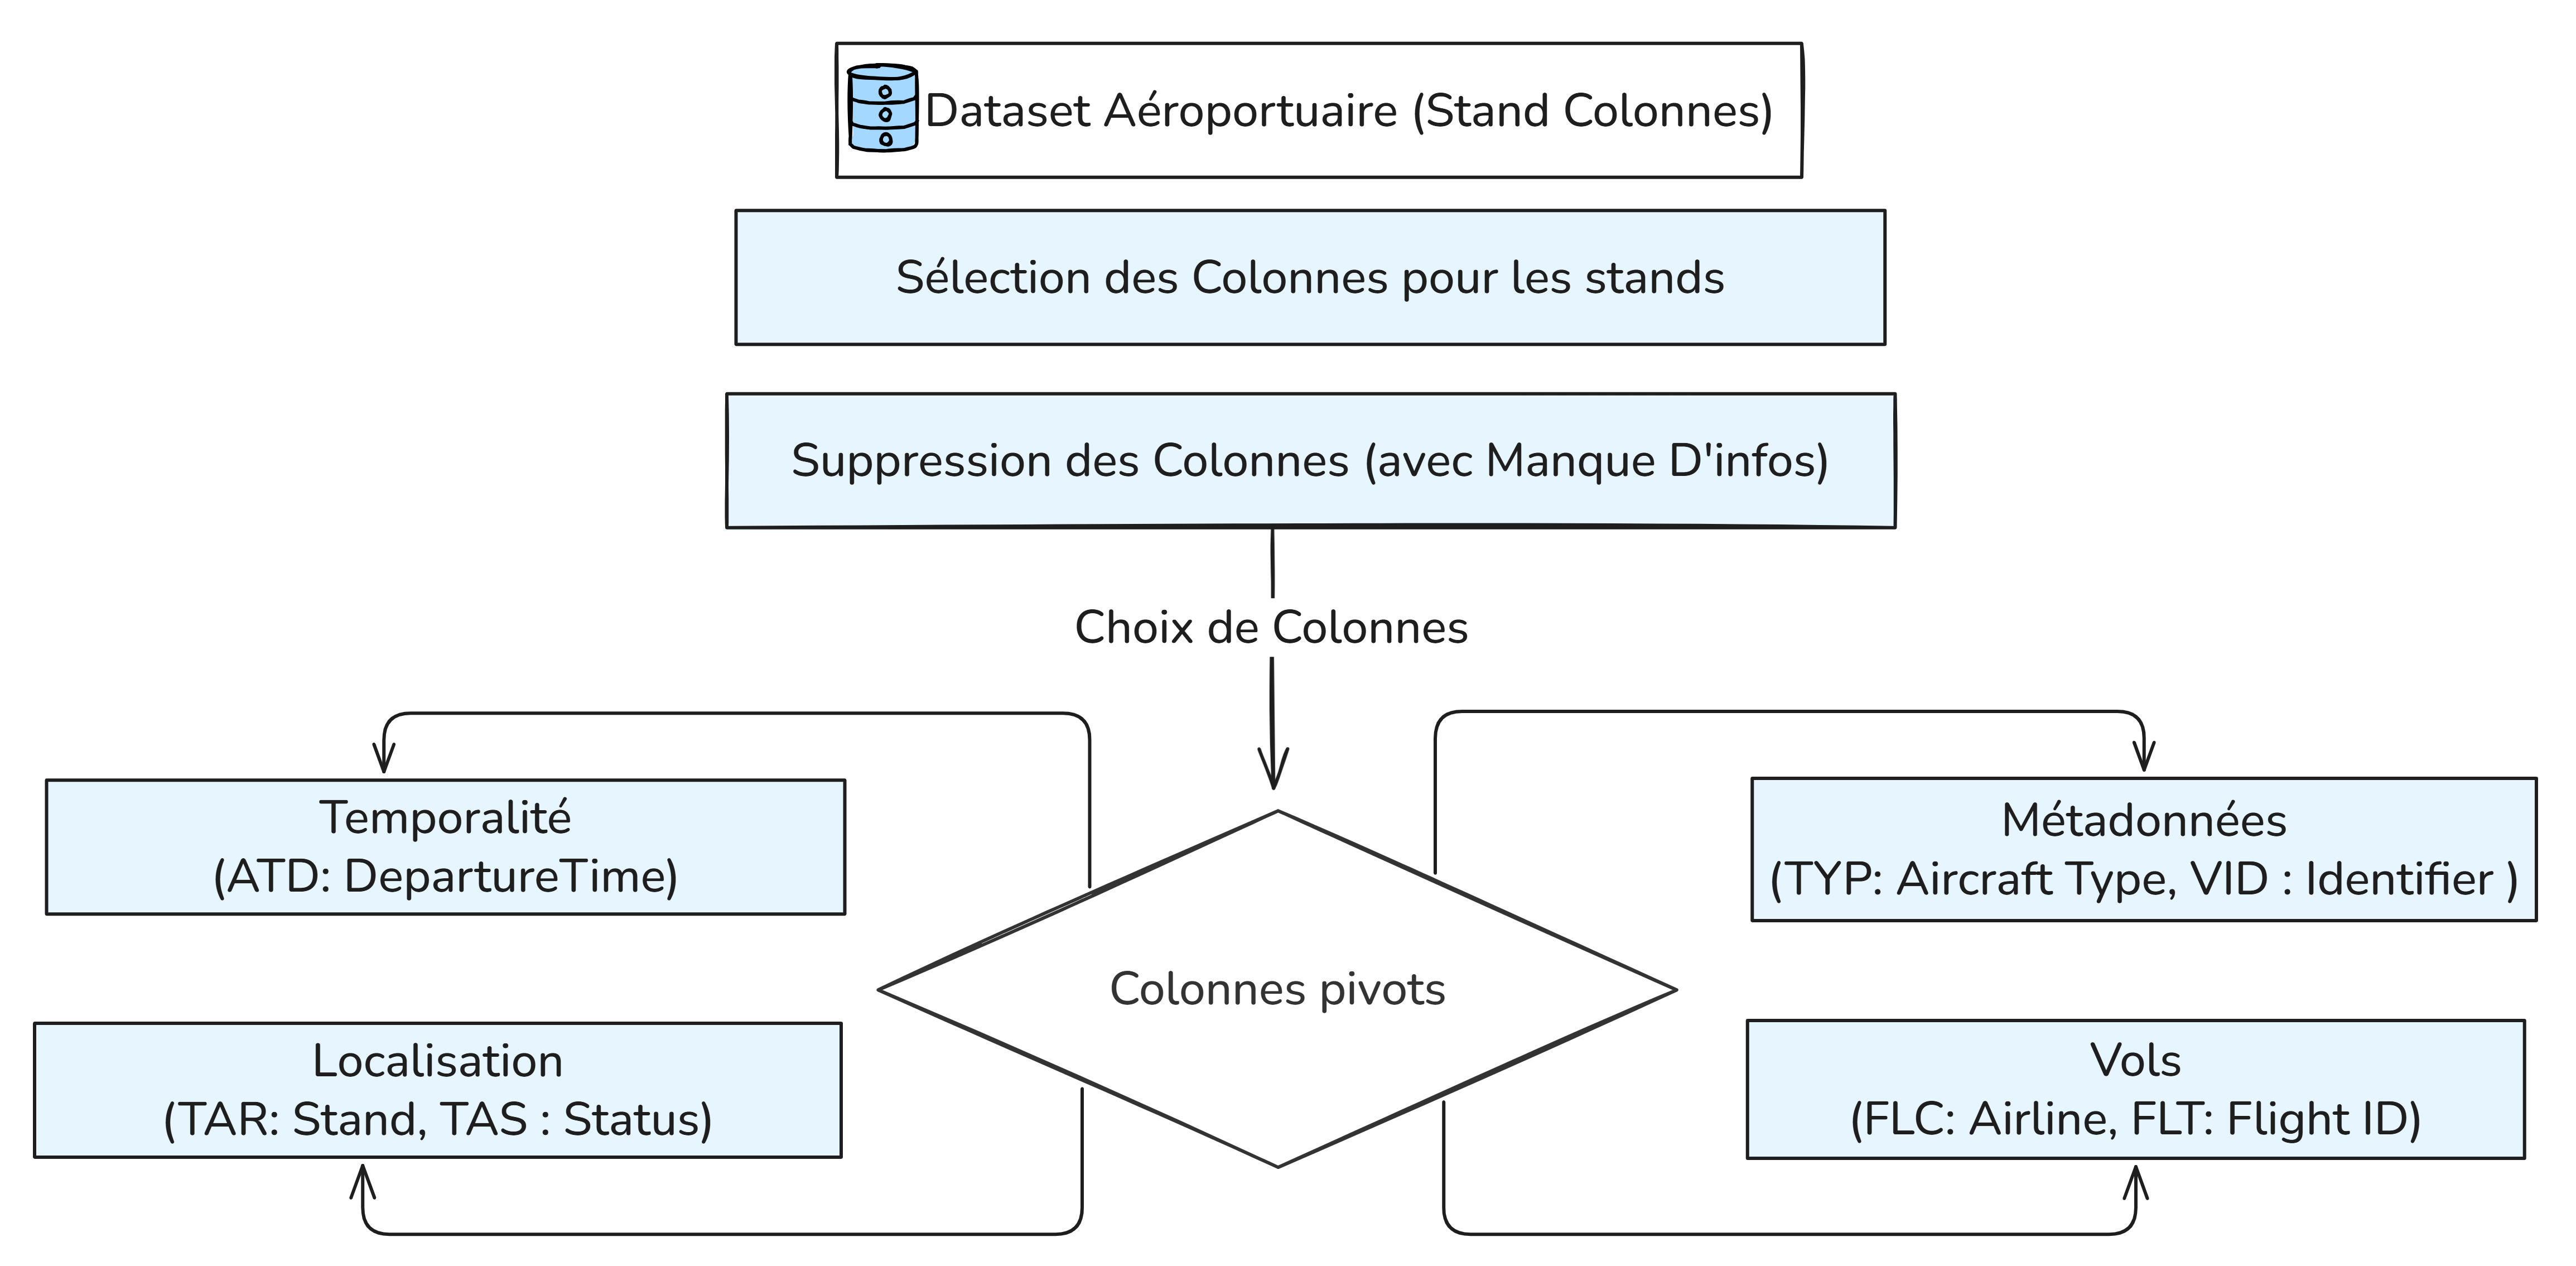
\includegraphics[width=0.8\linewidth]{assets/dataset/DataChart.jpg}
	\caption{Sélection des Caractéristiques}
	\label{fig:stand-selection}
\end{figure}

\subsubsection{Analyse des données}

Après avoir effectué la sélection des caractéristiques et le prétraitement, nous avons adopté une démarche analytique structurée, illustrée dans la figure~\ref{fig:stand-analysis-flow}. L’analyse a débuté par une vue d’ensemble des taux d’occupation des stands sur une période donnée, permettant d’identifier les tendances générales ainsi que le niveau d’utilisation de la capacité.

Pour une compréhension plus fine, l’analyse a ensuite été affinée en isolant chaque compagnie aérienne. Cela a permis de calculer les taux d’occupation des stands dédiés à chaque compagnie. Par la suite, nous avons évalué l’utilisation des stands par type d’avion au sein de chaque compagnie, afin de dégager des schémas liés à la catégorie d’appareil et à l’usage des infrastructures.

\begin{figure}[H]
	\centering
	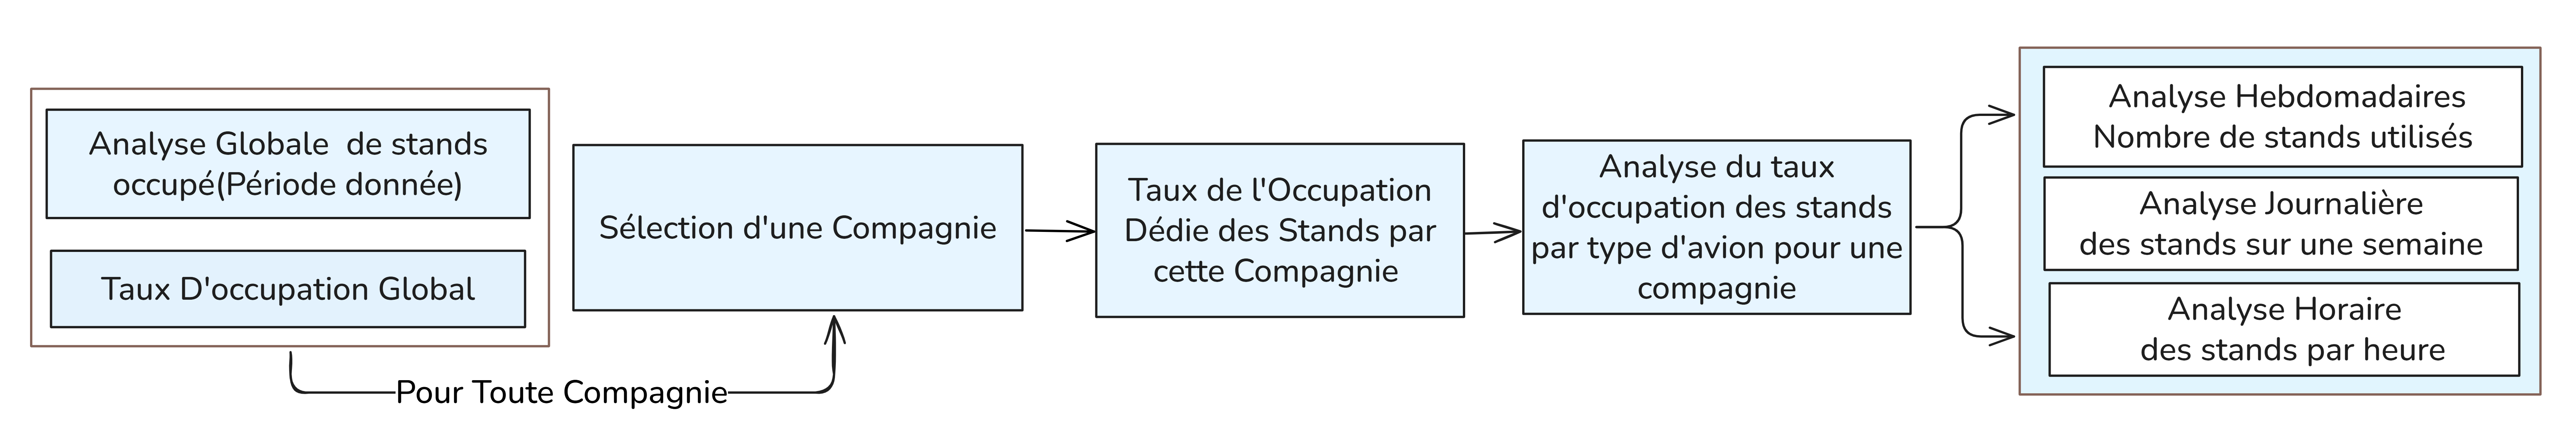
\includegraphics[width=1\linewidth]{assets/dataset/standAnalyse.png}
	\caption{Diagramme de Flux d'Analyse des Données}
	\label{fig:stand-analysis-flow}
\end{figure}


\begin{enumerate}
	\item \textbf{Analyse globale de l’occupation des stands}
	
	\hspace{0.5cm} Cette section présente une analyse approfondie de l’utilisation des postes de stationnement de l’aéroport sur une période de deux mois. L’objectif est d’identifier les schémas d’occupation en fonction des créneaux horaires et des compagnies aériennes, ainsi que d’évaluer l’efficacité de l’allocation des ressources selon les types d’avions.
	
	\begin{figure}[H]
		\centering
		\begin{subfigure}[t]{0.49\textwidth}
			\centering
			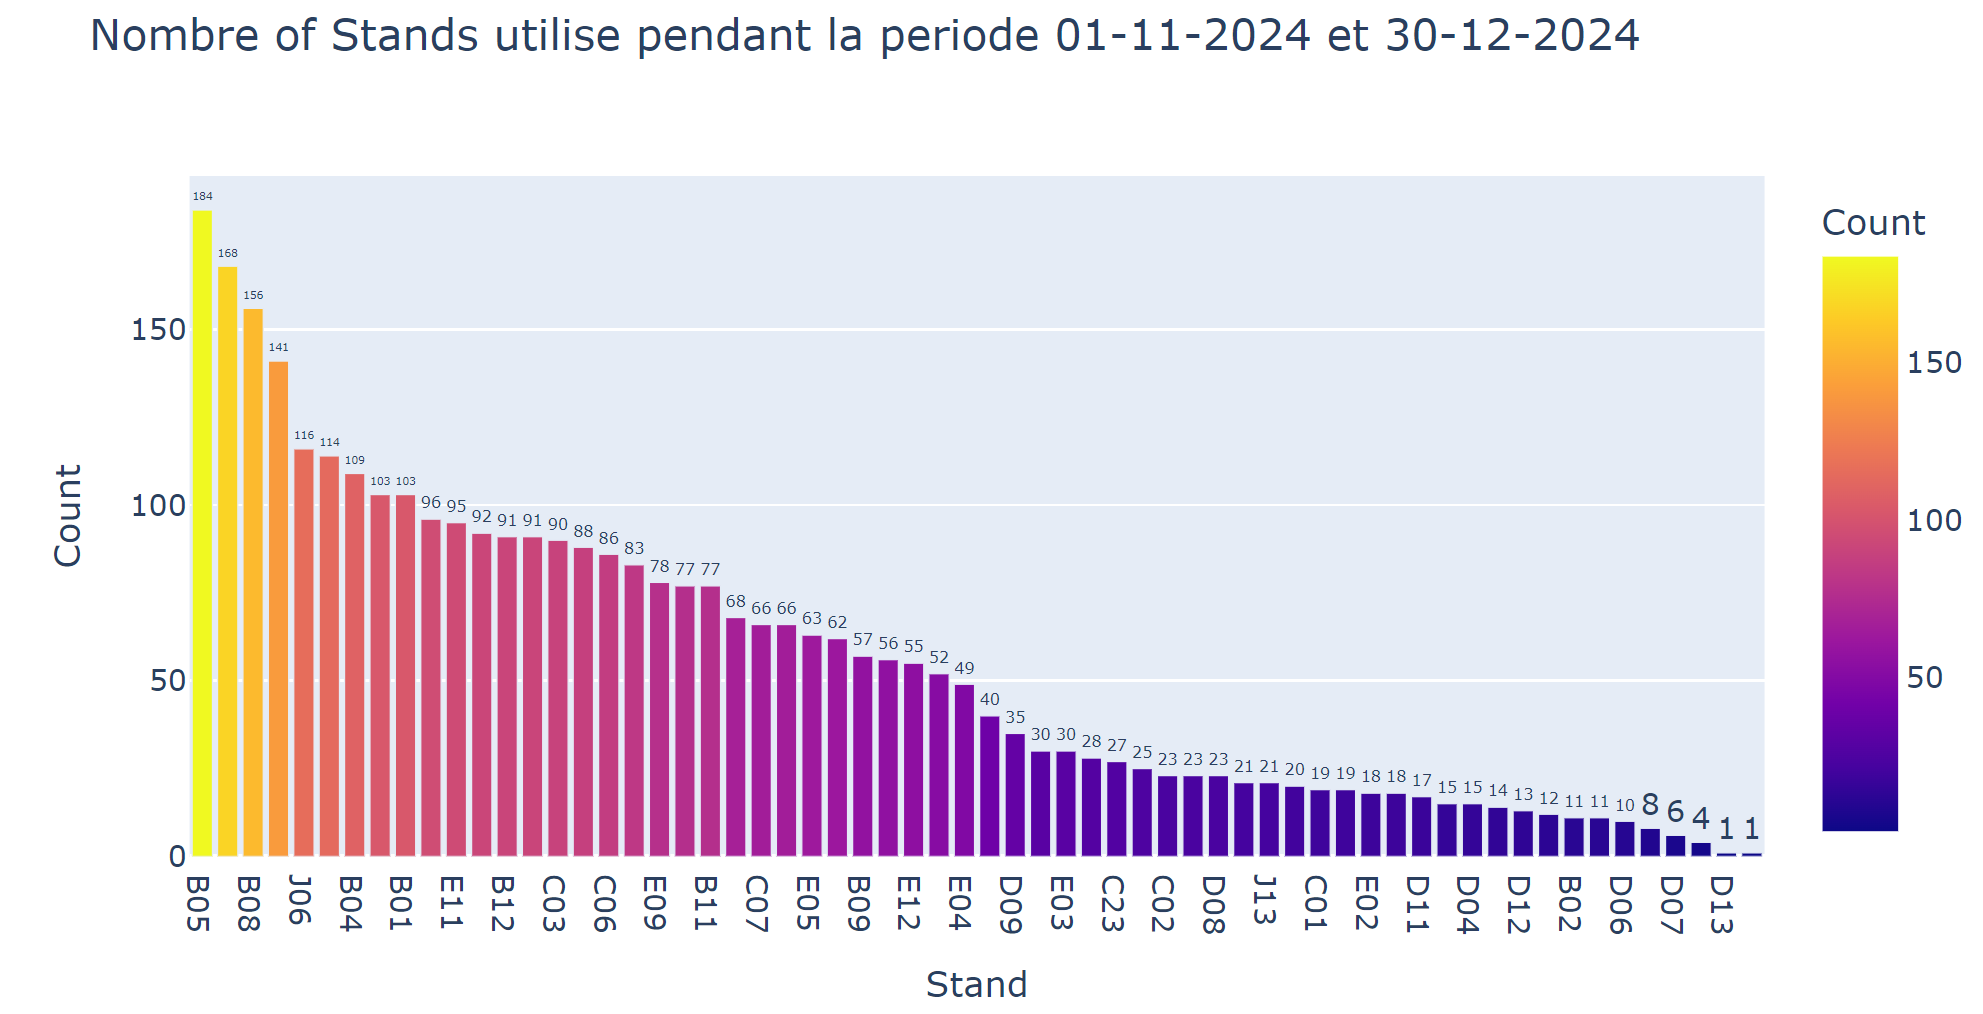
\includegraphics[width=\linewidth]{assets/dataset/Global_Satnds.png}
			\caption{Distribution de l'utilisation des stands sur la période d'étude (2 mois)}
			\label{fig:global_stands_utilization}
		\end{subfigure}
		\hfill
		\begin{subfigure}[t]{0.49\textwidth}
			\centering
			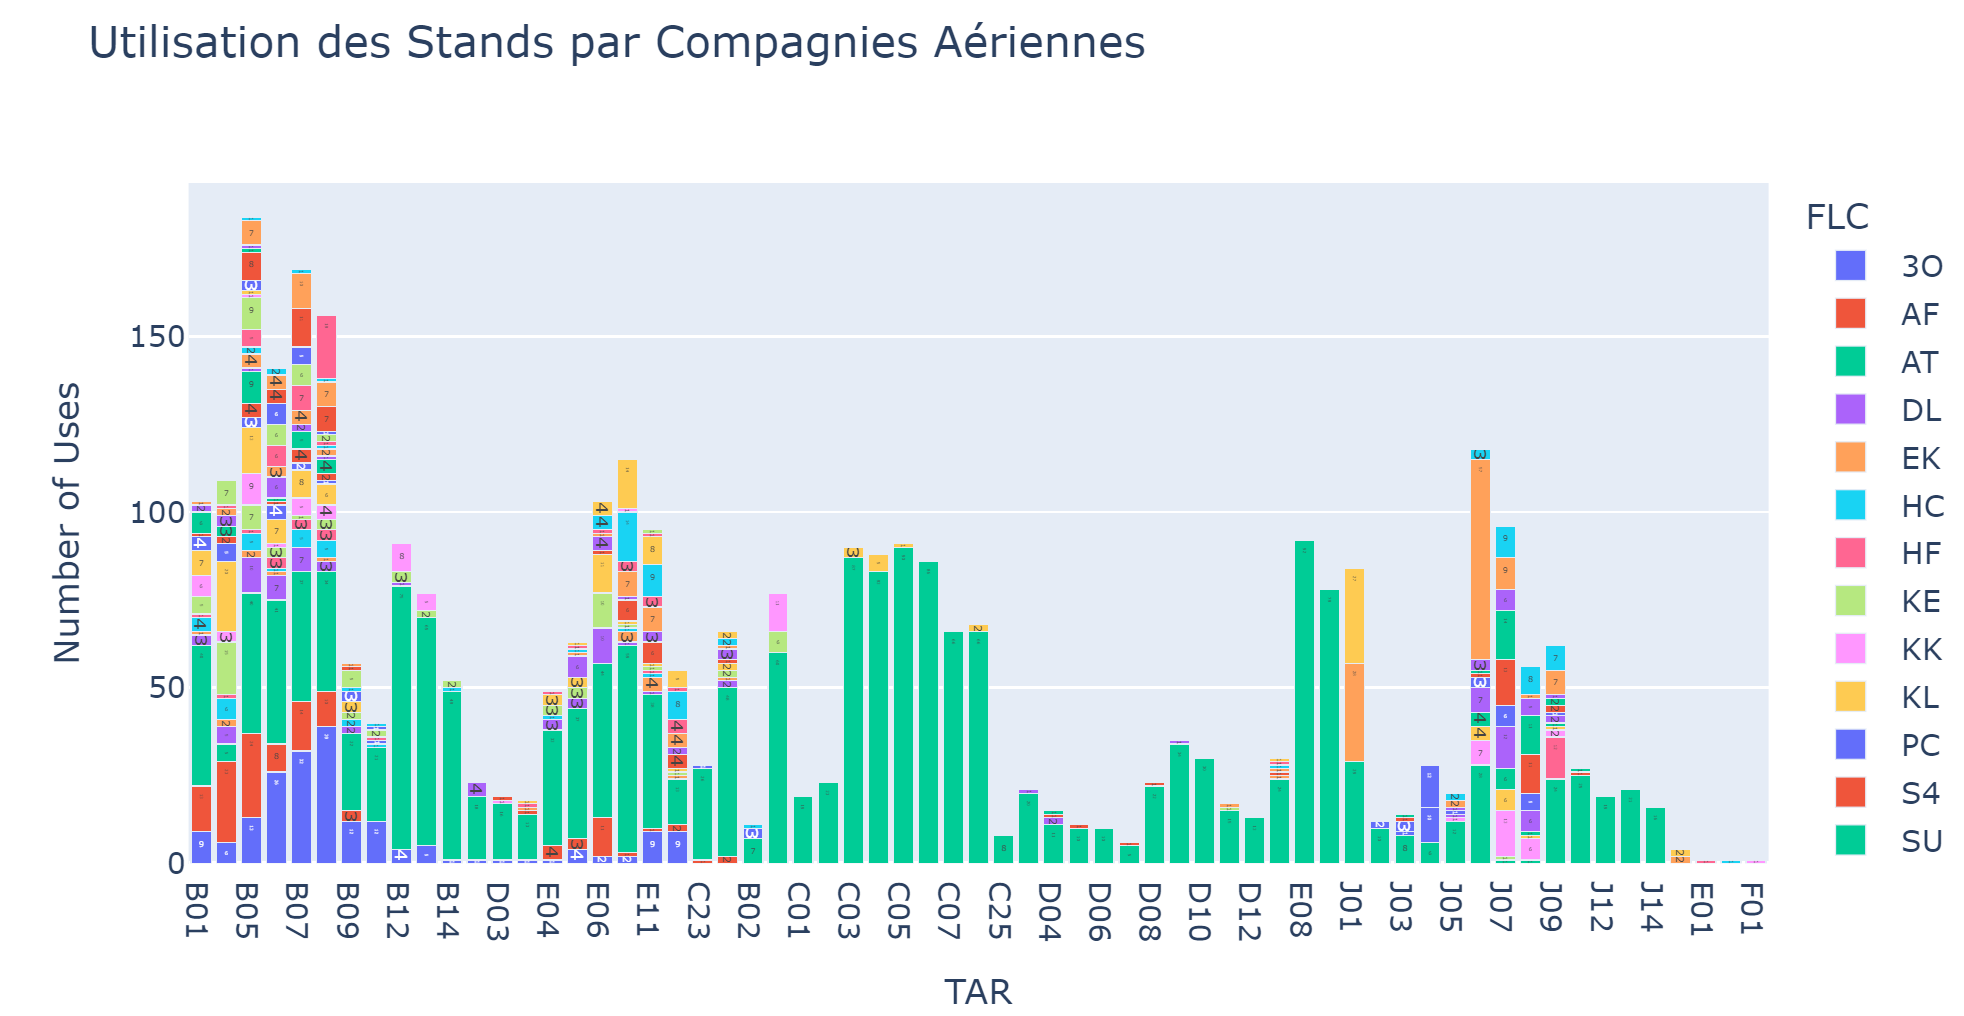
\includegraphics[width=\linewidth]{assets/dataset/Divsersity.png}
			\caption{Diversité des compagnies aériennes par stand}
			\label{fig:diversity_by_stand}
		\end{subfigure}
		\caption{Diversité des compagnies aériennes par stand}
		
	\end{figure}
	
	

	\hspace{0.5cm} La \textbf{figure \ref{fig:global_stands_utilization}} met en évidence une répartition hétérogène de l’occupation des stands. Certaines positions de stationnement présentent des taux d’occupation nettement supérieurs à la moyenne, notamment :  
	\textbf{B05 (184), B07 (168), B08 (156), B06 (141) et J06 (116).}
	
	À l’inverse, certains stands sont très peu utilisés :  
	\textbf{D07 (6), J15 (4), D13 (1) et E01 (1).}
L’emplacement physique de ces stands sur le plan de l’aéroport est présenté en \textbf{annexe} (voir Figure~\ref{fig:plan}).

	\hspace{0.5cm} La \textbf{figure de droite~\ref{fig:diversity_by_stand}} illustre la diversité des compagnies aériennes par stand. Elle montre que certains emplacements accueillent une large variété de transporteurs. Par exemple, le \textbf{stand B01} est utilisé par au moins \textbf{cinq compagnies différentes} (\ac{3O}, AF, \ac{AT}, DL, EK) avec des fréquences variables.
	
	\item \textbf{Utilisation des stands par compagnie aérienne et type d’avion}
	
	\hspace{0.5cm} Cette section examine en détail l’utilisation des stands, en se concentrant sur deux aspects : la répartition par compagnie aérienne et par type d’avion. L’objectif est d’identifier les principaux utilisateurs des infrastructures aéroportuaires et de comprendre la répartition des types d’appareils.
	
	\begin{figure}[H]
		\centering
		\begin{minipage}[b]{0.52\linewidth}
			\centering
			\includegraphics[width=\linewidth]{assets/dataset/compagnie.png}
			\caption{Répartition de l'occupation des stands par compagnie aérienne}
			\label{fig:airline_occupation}
		\end{minipage}
		\hfill
		\begin{minipage}[b]{0.45\linewidth}
			\centering
			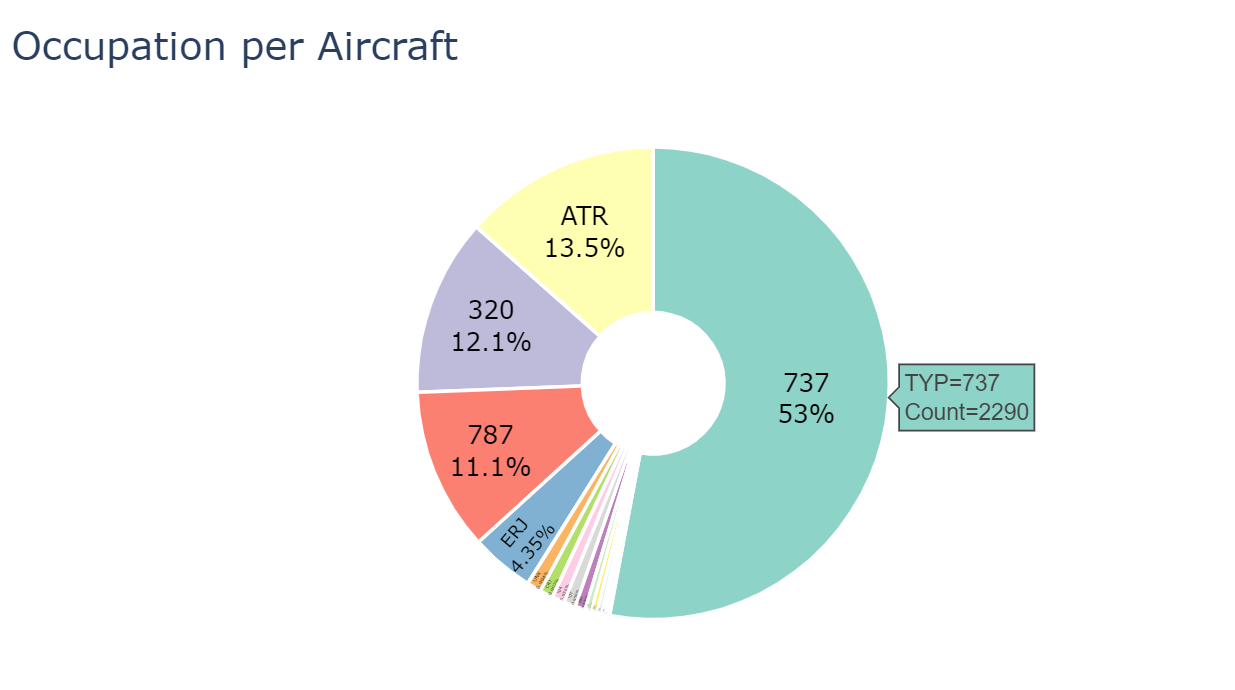
\includegraphics[width=\linewidth]{assets/dataset/AircraftOccupation.png}
			\caption{Répartition de l’occupation par type d’avion}
			\label{fig:AicraftOccupation}
		\end{minipage}
	\end{figure}
	
\hspace{0.5cm} \textbf{La figure de gauche~\ref{fig:airline_occupation}} révèle une prédominance marquée des transporteurs nationaux marocains. Notamment, \ac{AT} représente une part importante de l’utilisation des stands.

\begin{table}[H]
	\centering
	\renewcommand{\arraystretch}{0.8} % réduit l'espacement vertical
	\caption{Principales compagnies aériennes selon le nombre d’utilisations des stands}
	\begin{tabular}{l l c}
		\toprule
		\textbf{Code IATA} & \textbf{Compagnie} & \textbf{Nombre d’utilisations} \\
		\midrule
		AT & Royal Air Maroc & 3361 \\
		3O & Air Arabia Maroc & 221 \\
		AF & Air France & 122 \\
		AC & Air Canada & 47 \\
		6E & IndiGo & 29 \\
		\bottomrule
	\end{tabular}
	\label{tab:top_airlines}
\end{table}


\hspace{0.5cm} Cette distribution confirme la domination de \ac{AT}, suivie par \ac{3O}, indiquant que les compagnies nationales sont les principaux utilisateurs des infrastructures aéroportuaires.

\hspace{0.5cm} \textbf{La figure de droite~\ref{fig:AicraftOccupation}} montre que trois types d’avions dominent les opérations aéroportuaires : le Boeing 737 (46,6 \%), l’Airbus A320 (16,7 \%) et l’ATR (12,2 \%). Ensemble, ils représentent plus de 75 \% des mouvements totaux. Des appareils comme le Boeing 787 (11,9 \%) et l’Embraer ERJ (4,6 \%) sont modérément utilisés, tandis que d’autres types sont marginalement présents.

\item \textbf{Analyse selon trois niveaux de fréquence}

\hspace{0.5cm} L’étude des tendances temporelles de l’occupation des stands permet d’identifier les schémas cycliques et saisonniers qui caractérisent les opérations aéroportuaires. Cette analyse multiniveau offre une compréhension détaillée des variations de la demande en stands au fil du temps.

\begin{figure}[H]
	\centering
	\begin{minipage}[b]{0.49\linewidth}
		\centering
		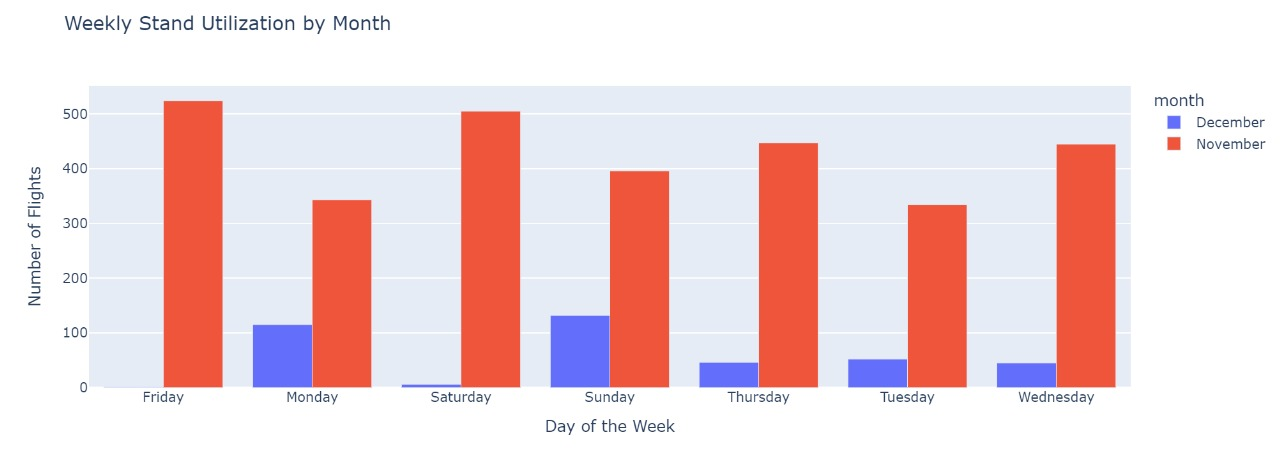
\includegraphics[width=\linewidth]{assets/dataset/WeeklyOccupation.jpg}
		\caption{Variation hebdomadaire de l’occupation des stands}
		\label{fig:WeeklyOccupation}
	\end{minipage}
	\hfill
	\begin{minipage}[b]{0.49\linewidth}
		\centering
		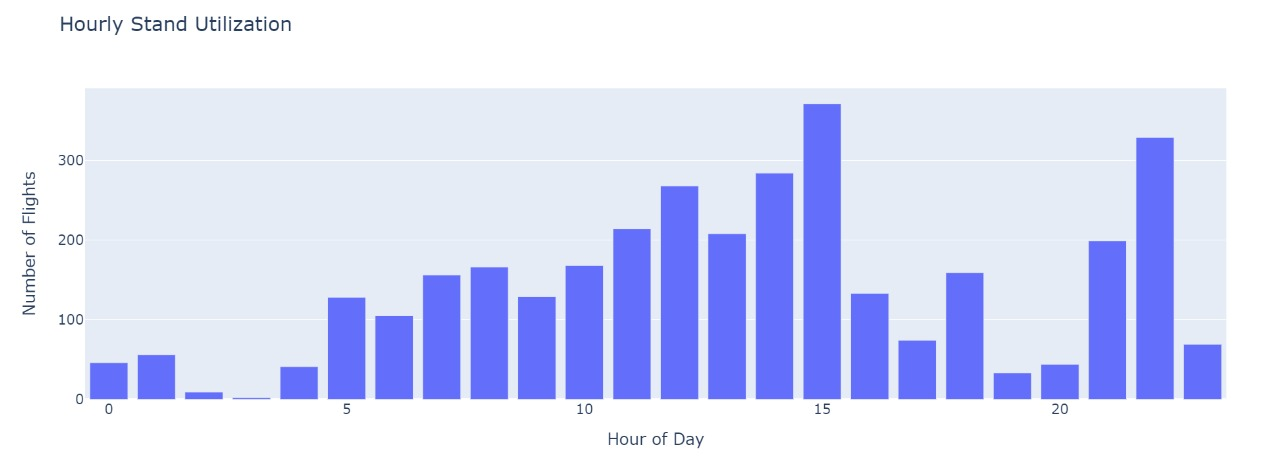
\includegraphics[width=\linewidth]{assets/dataset/HourlyOccupation.jpg}
		\caption{Variation horaire de l’occupation des stands}
		\label{fig:HourlyOccupation}
	\end{minipage}
\end{figure}

\hspace{0.5cm} \textbf{Gauche : Analyse hebdomadaire \ref{fig:WeeklyOccupation}}
Cette analyse met en évidence des tendances hebdomadaires et saisonnières d’occupation. En novembre, les pics sont observés le vendredi (524 vols), samedi (505) et dimanche (396), indiquant une forte activité en fin de semaine. En décembre, l’activité diminue globalement, avec des pics plus modestes le dimanche (132) et le lundi (115).  


\hspace{0.5cm} \textbf{Droite : Analyse horaire \ref{fig:HourlyOccupation}}
Cette analyse révèle que l’activité est concentrée entre 5h et 16h, avec des pics à 15h (371 vols), 14h (284) et un second à 22h (329), probablement lié aux départs tardifs. L’activité est minimale entre 2h et 4h du matin.


\end{enumerate}





\subsection{Analyse des retards}

L’analyse des retards représente un volet important de notre étude, car elle permet de mieux comprendre les sources de perturbations et leur impact sur la planification des stands.

Comme illustré dans la Figure~\ref{fig:retard_flowchart}, cette analyse débute par un prétraitement des données, visant à nettoyer, filtrer et structurer les informations relatives aux retards. Ensuite, plusieurs visualisations globales sont produites.

Par ailleurs, nous avons approfondi l’étude en catégorisant les retards selon différents axes :

\begin{itemize}
\item Retards par compagnie aérienne.
\item Niveau de criticité par compagnie.
\item Retards en fonction du stand utilisé.
\item Retards selon la taille de l'avion.
\end{itemize}

\begin{figure}[H]
\centering
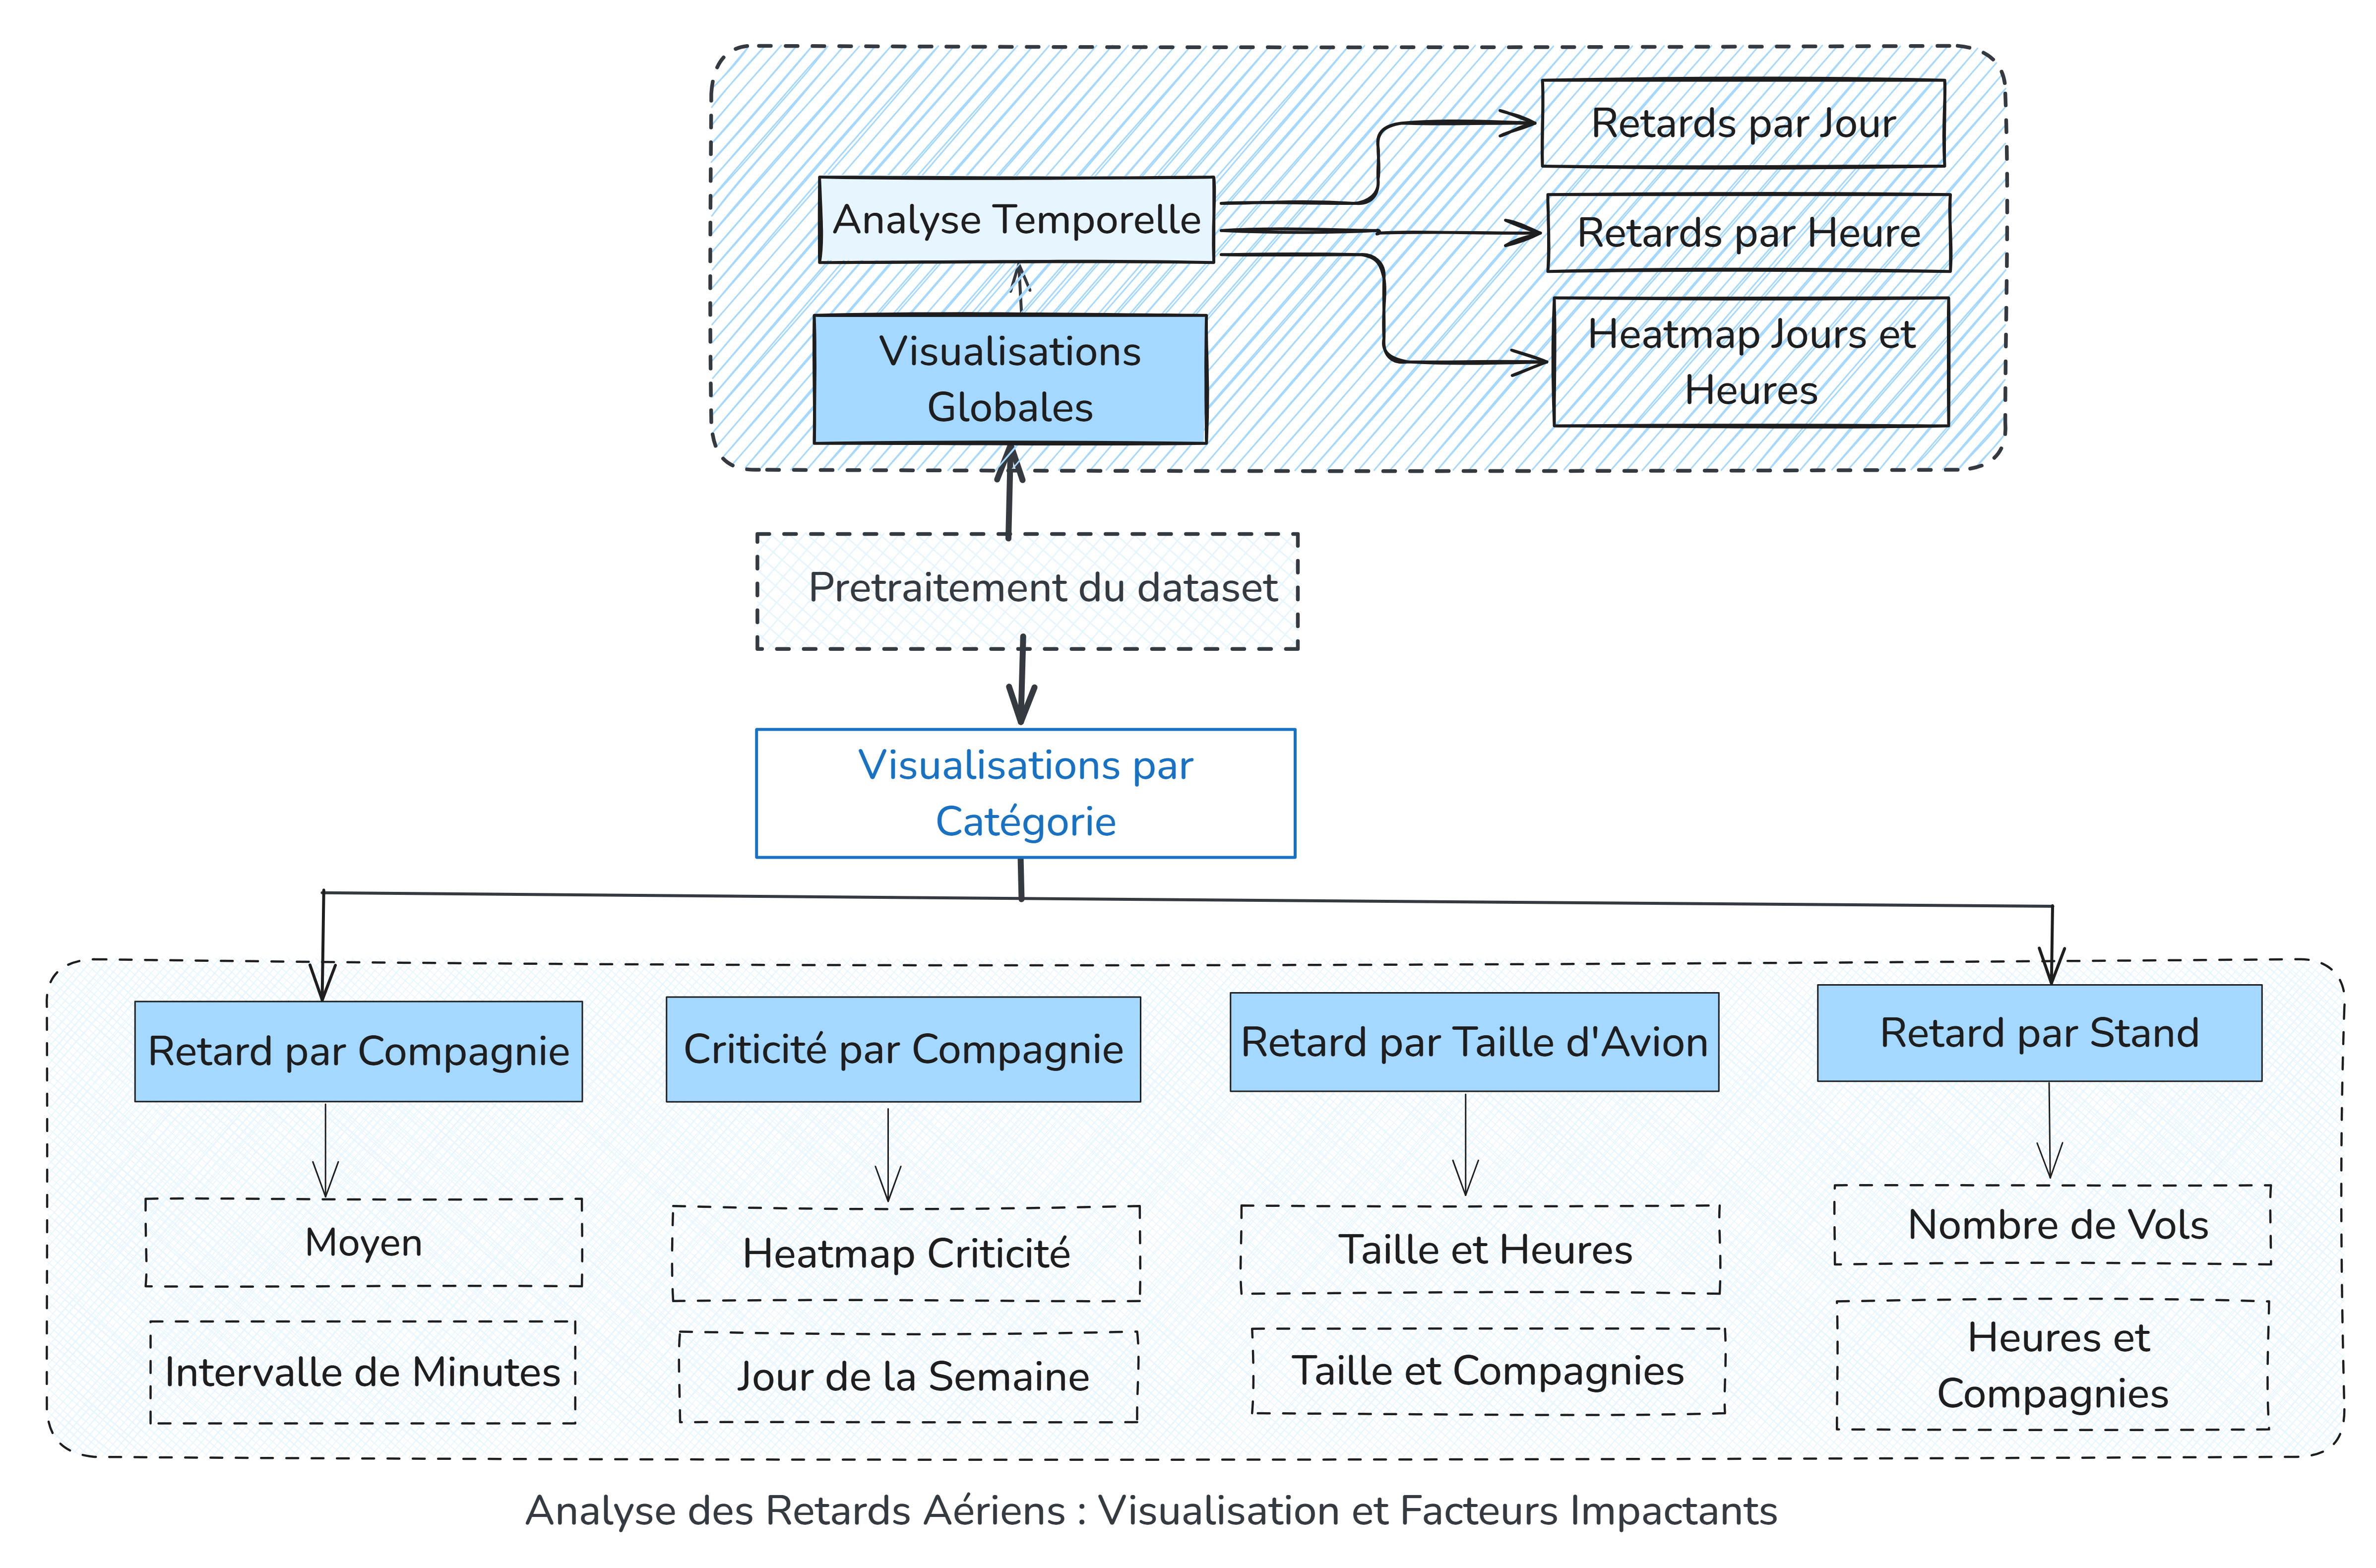
\includegraphics[width=0.9\linewidth]{assets/dataset/flowchartRetard.png}
\caption{Flowchart de l'analyse des retards}
\label{fig:retard_flowchart}
\end{figure}
Les résultats obtenus permettent d’identifier les sources potentielles de saturation ou de mauvaise allocation des ressources aéroportuaires, et servent de base pour générer un dataset optimisé destiné à l’apprentissage de notre modèle de prédiction et d’affectation des stands.

\subsubsection{Prétraitement du dataset}
Cette section décrit les \textbf{étapes clés du prétraitement} effectuées sur notre dataset pour l’analyse des retards aériens.
\begin{figure}[H]
\centering
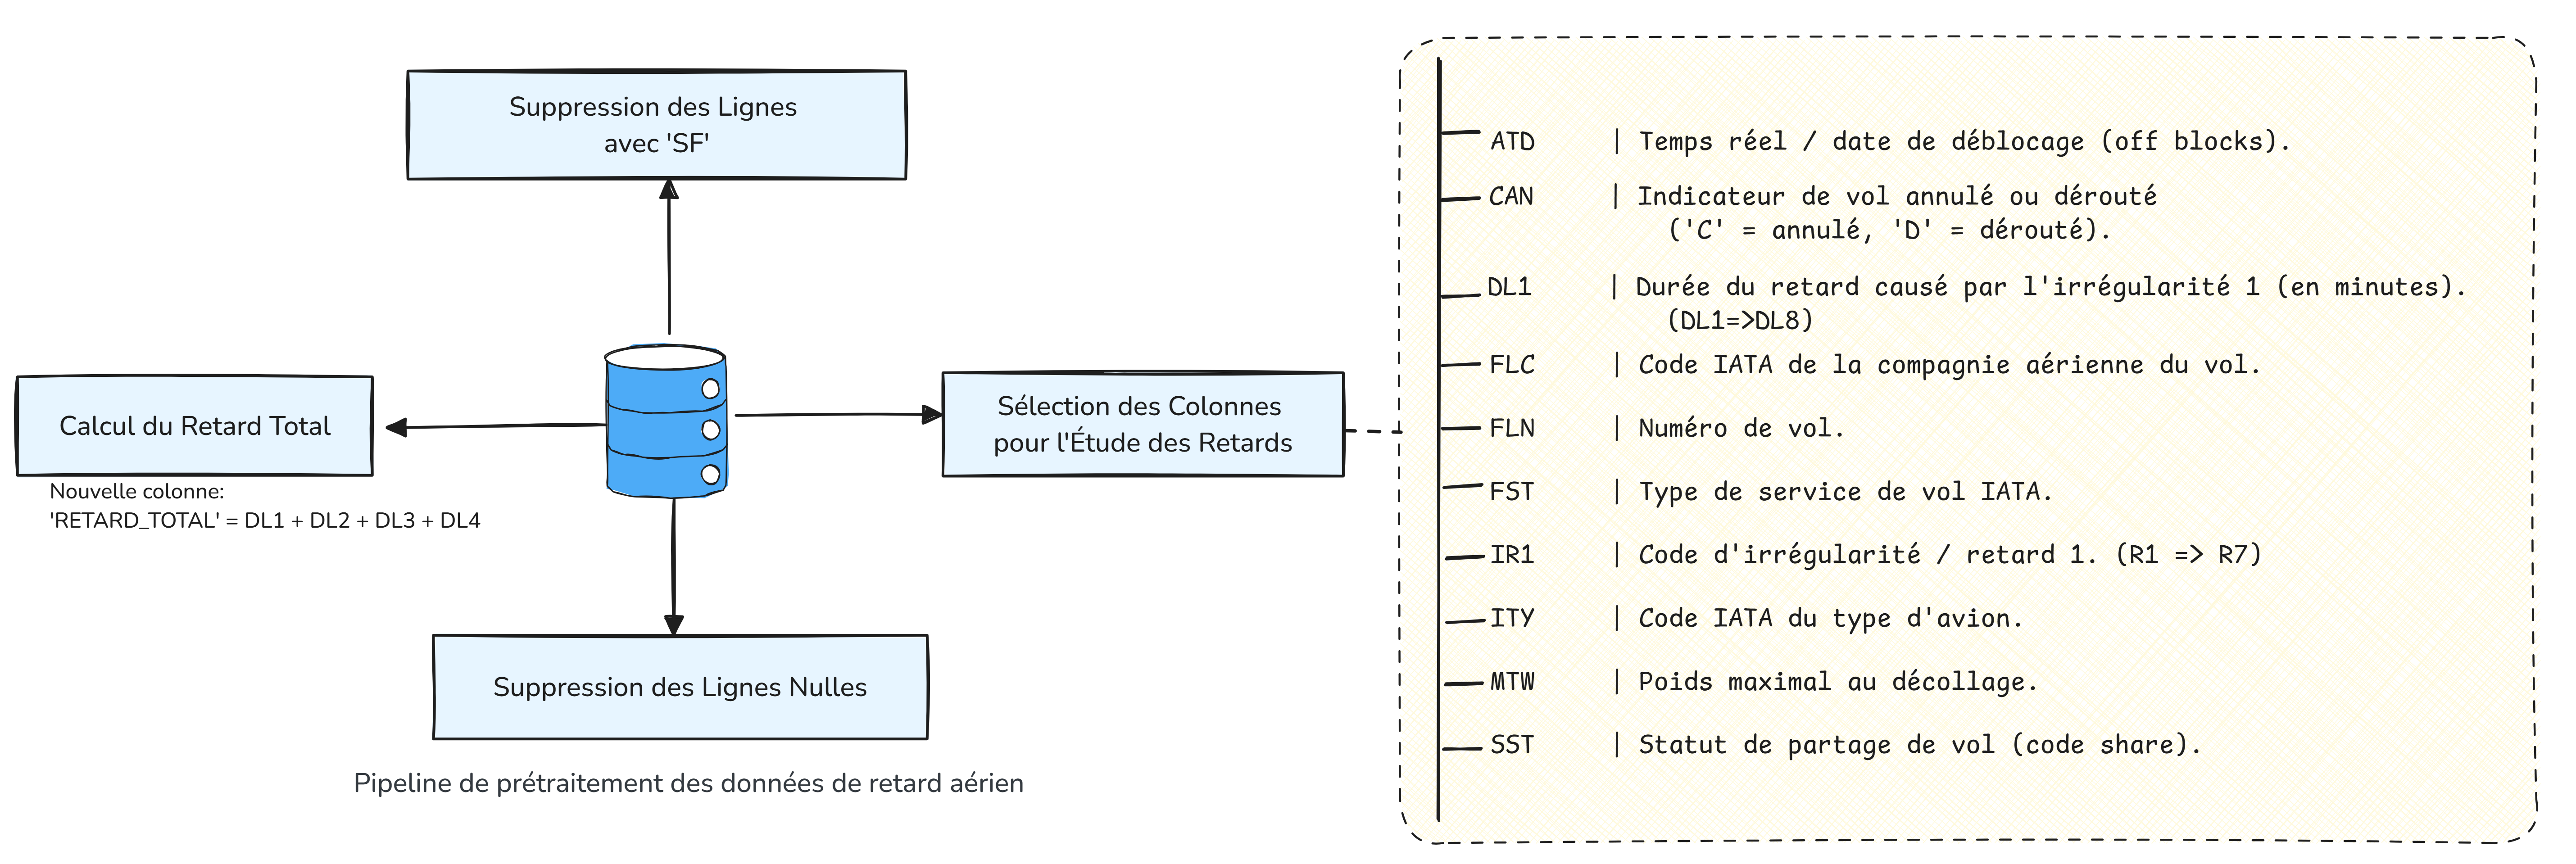
\includegraphics[width=0.8\linewidth]{assets/dataset/pretraitement.png}
\caption{Les étapes de prétraitement du dataset}
\label{fig:pretraitementData}
\end{figure}

Ces étapes ont été définies à partir d’une \textbf{étude approfondie du document de référence} fourni par le client, documentant en détail les \textbf{485 colonnes} disponibles dans le fichier source. L’objectif était de filtrer et structurer les données de manière à isoler les variables les plus pertinentes pour l’étude des retards.

\vspace{0.5em}
\textbf{1. Sélection stratégique des colonnes}

Sur la base du document PDF fourni par le client, une sélection des colonnes a été effectuée pour l’analyse des retards. Les variables retenues incluent :

\begin{itemize}
\item \texttt{ATD}: Représente l’heure réelle de départ du vol, essentielle pour le calcul précis du retard.

\item \texttt{CAN} : Indicateur précisant si un vol a été annulé ou dérouté.

\item \texttt{IR1} à \texttt{IR8} : Ensemble de colonnes représentant les causes détaillées des retards (problèmes techniques, météo, trafic, etc.) sous forme de codes.

\item \texttt{DL1} à \texttt{DL8} : Durée du retard (en minutes) associée à chaque cause pour un vol donné.

\item \texttt{MTW}: Poids maximal autorisé pour le décollage de l’avion.

\item \texttt{SST} : Indicateur du statut de partage de vol (code-share).
\end{itemize}


\vspace{0.5em}
\textbf{2. Nettoyage des données}

Une fois les colonnes pertinentes sélectionnées, nous avons entrepris un nettoyage du dataset :

\begin{itemize}
\item \textbf{Suppression des lignes incomplètes} : Toutes les entrées contenant des valeurs nulles dans les colonnes.
\item \textbf{Filtrage des vols non pertinents} : En se basant sur l'analyse des vols lors de l’étude initiale, les lignes où
certaines compagnies n’opéraient que des vols en partage de code, sans présence opérationnelle directe ont été écartées.
\end{itemize}

\vspace{0.5em}
\textbf{3. Création de la colonne \texttt{RETARD\_TOTAL}}

D'après les indications fournies par le client, la durée totale de retard correspond à la somme des retards enregistrés. Alors, la variable \texttt{RETARD\_TOTAL} agrège les minutes de retard signalées dans les colonnes \texttt{DL1} à \texttt{DL8}. La formule utilisée est la suivante :

\[
\texttt{RETARD\_TOTAL} = \sum_{i=1}^{8} \texttt{DL}_i
\]




\subsubsection{Visualisations globales}
Des visualisations globales ont été réalisées pour mieux comprendre le comportement du dataset.
\paragraph{Retards par jour et par heure}
\mbox{}\\
La figure \ref{fig:retards_temporels} présente deux visualisations : la première montre le nombre de vols retardés par jour, tandis que la seconde illustre le pourcentage de retards en fonction de l’heure de la journée.
\begin{figure}[H]
\centering
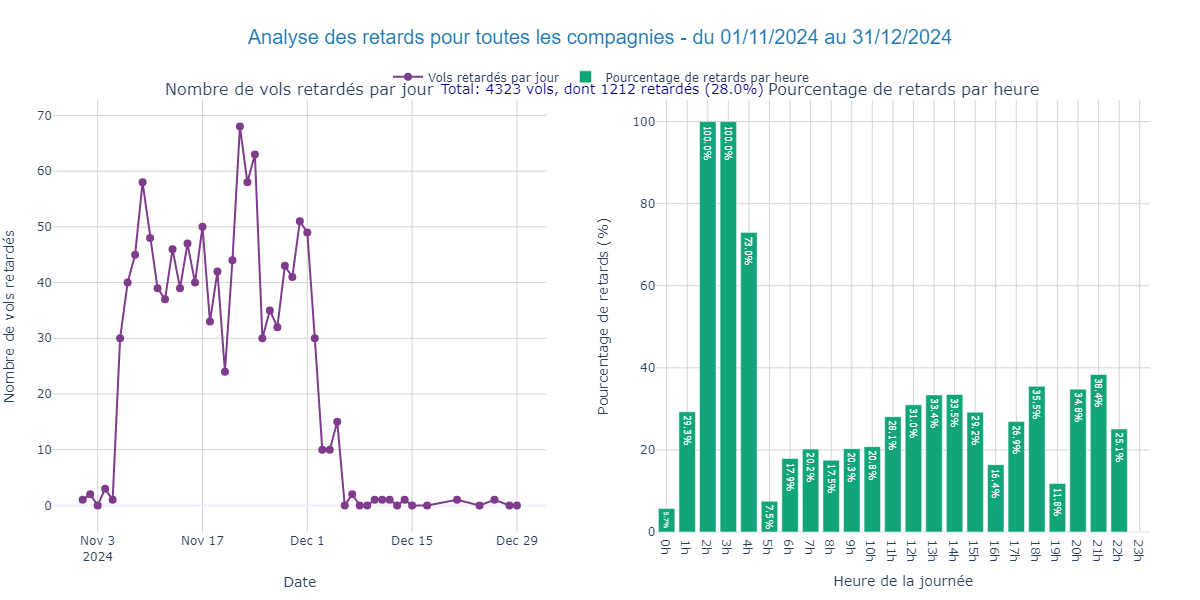
\includegraphics[width=0.9\linewidth]{assets/dataset/parCompagnie.png}
\caption{Analyse temporelle des retards : par jour et par heure}
\label{fig:retards_temporels}
\end{figure}
\vspace{-1em}
Nous analysons la répartition temporelle des vols retardés sur l’ensemble de la période d’étude.Le mois de novembre montre une concentration élevée de retards, avec des pics dépassant 60 vols par jour. La diminution en décembre s'explique par la répartition du trafic aérien où l'\ac{CMN} enregistre moins de vols durant cette période, tandis que l'aéroport de Marrakech devient dominant.

\vspace{-1em}
\paragraph{Analyse des retards par période et par stand}
\mbox{}\\
Cette section présente une double analyse des retards enregistrés entre novembre et décembre 2024, en croisant les données selon les jours/heures et les stands d’affectation.
 \vspace{-1em}
\begin{figure}[H]
	\centering
	\begin{subfigure}[b]{0.5\textwidth}
		\centering
		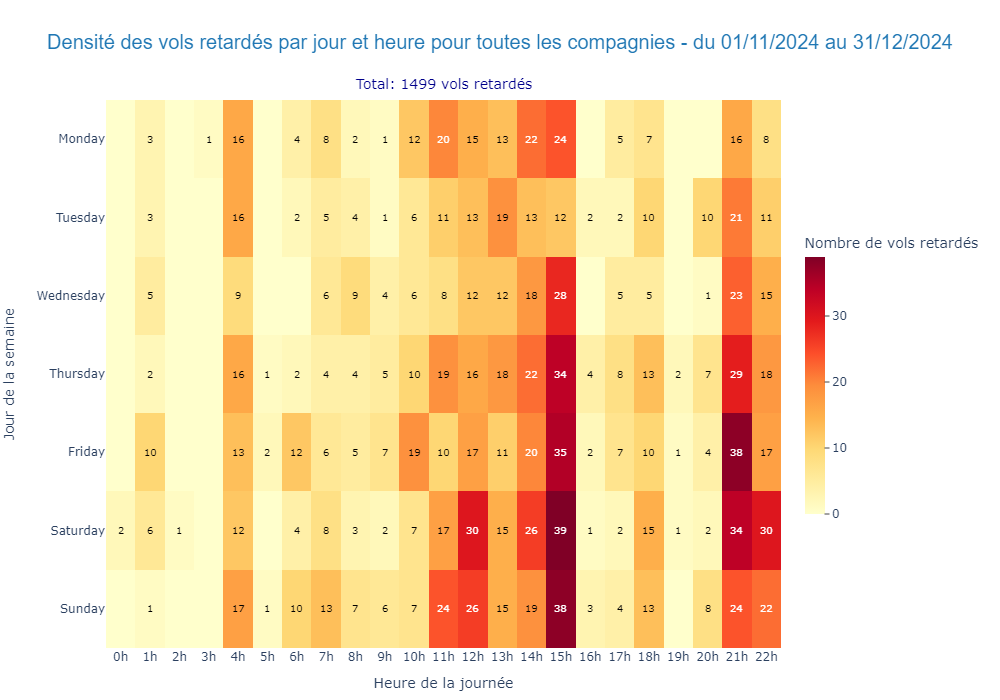
\includegraphics[width=\linewidth]{assets/dataset/parComapgnie2.png}
		\caption{Retards par jour de la semaine et heure (Nov–Déc 2024)}
		\label{fig:heatmap_retards}
	\end{subfigure}
	\hfill
	\begin{subfigure}[b]{0.48\textwidth}
		\centering
		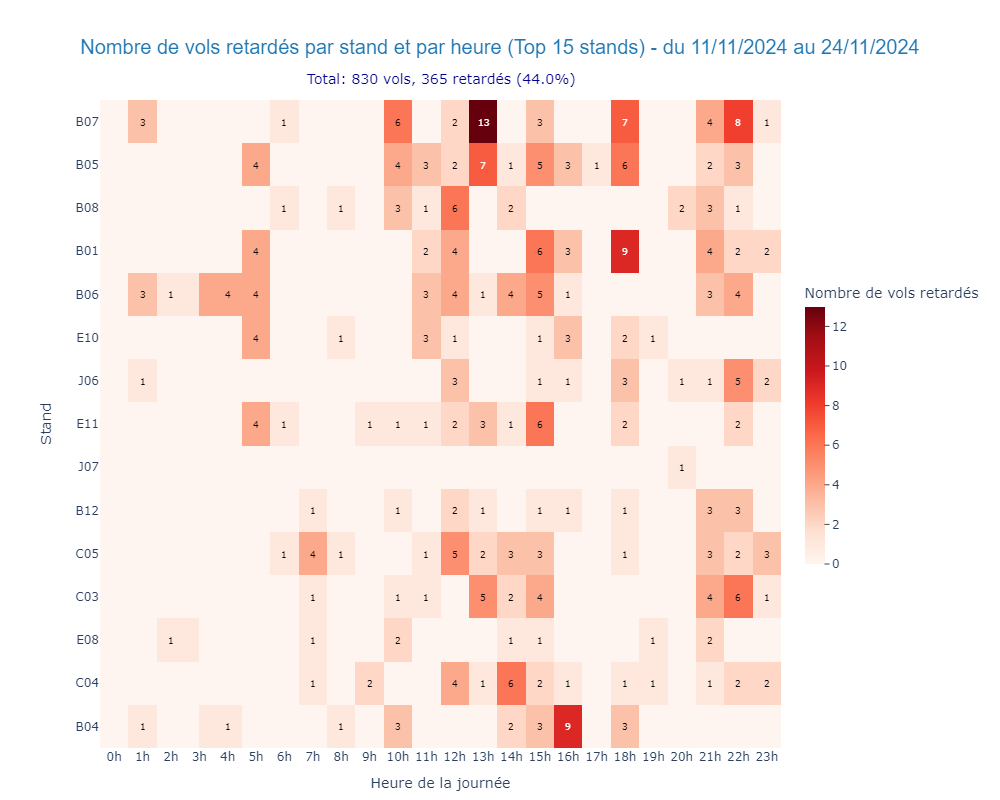
\includegraphics[width=\linewidth]{assets/dataset/parStand.png}
		\caption{Retards par stand et heure (11–24 nov. 2024)}
		\label{fig:retard_stand}
	\end{subfigure}
	\caption{Analyse croisée des retards selon différentes dimensions}
\end{figure}
 \vspace{-1em}
Les résultats montrent des pics de retards :
\begin{itemize}[leftmargin=1.5em]
	\item Le \textbf{vendredi}, le \textbf{samedi après-midi} et le \textbf{dimanche soir}, en lien avec le trafic hebdomadaire.
	\item Aux stands \textbf{B07}, \textbf{B05} et \textbf{B01}, surtout entre \textbf{11h et 16h}, où l’activité est particulièrement dense.
\end{itemize}
 \vspace{-1em}
\subsubsection{Visualisations par catégorie}
 \vspace{-0.5em}
Des visualisations par catégorie ont été réalisées pour approfondir l’analyse. 
\begin{enumerate}
	\item \textbf{Retard par compagnie}
	
	Cette section explore la criticité des retards selon les compagnies aériennes, les jours de la semaine et les créneaux horaires.
	
	\begin{figure}[H]
		\centering
		\begin{subfigure}[b]{0.5\linewidth}
			\centering
			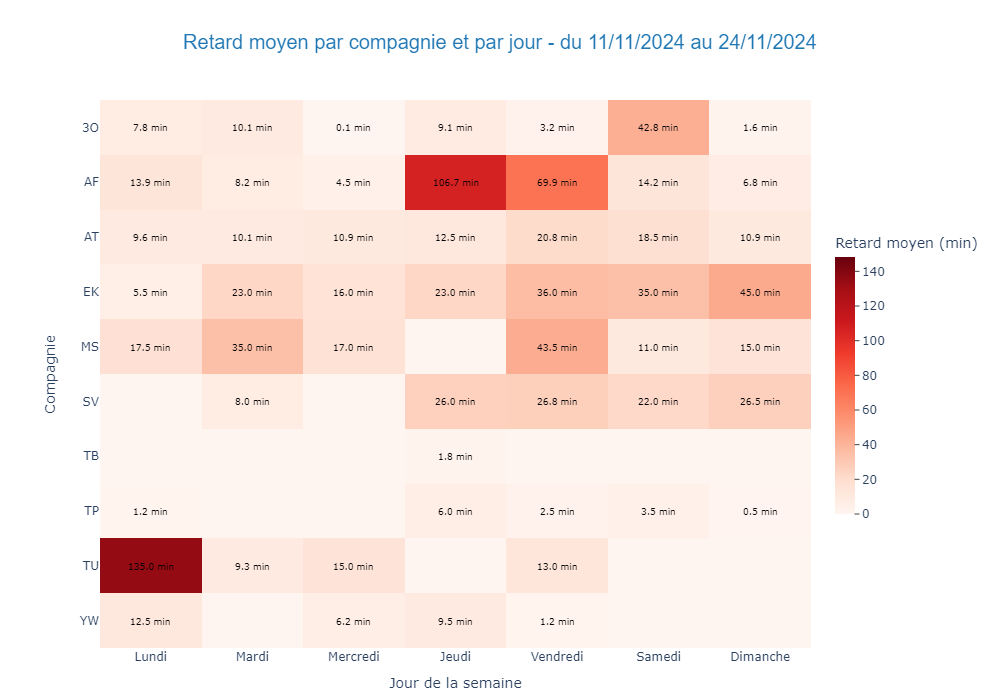
\includegraphics[width=\linewidth]{assets/dataset/parCompagnie3.png}
			\caption{Retard moyen (en min) par compagnie et par jour}
			\label{fig:retard_par_jour}
		\end{subfigure}
		\hfill
		\begin{subfigure}[b]{0.48\linewidth}
			\centering
			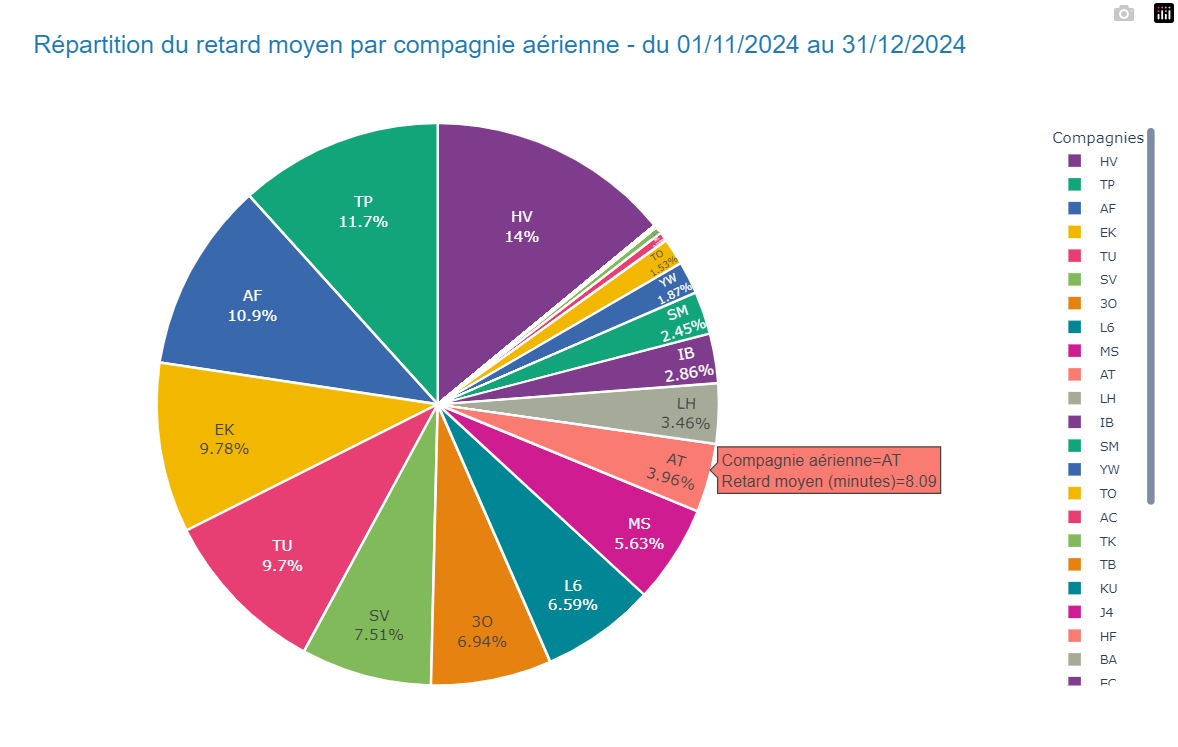
\includegraphics[width=\linewidth]{assets/dataset/parCompagnie4.png}
			\caption{Répartition globale du retard moyen par compagnie}
			\label{fig:repartition_retard}
		\end{subfigure}
		\caption{Visualisations des retards moyens selon les compagnies aériennes}
		\label{fig:retards_par_compagnie}
	\end{figure}
\vspace{-1.6em}
La heatmap \ref{fig:retard_par_jour} montre par exemple un pic critique pour \textbf{TU (Tunisair)} le lundi (135 min). D'autres compagnies comme \textbf{AF} ou \textbf{MS (EgyptAir)} présentent également des retards élevés.  
Le graphique circulaire (\ref{fig:repartition_retard}) indique que \textbf{Transavia} enregistre le retard moyen le plus élevé (14\%), tandis que \textbf{\ac{AT}} affiche un retard moyen faible (8 min).
 \vspace{-1em}
\paragraph{Criticité par jour et par heure}  

 \vspace{-0.5em}
Cette analyse croise les compagnies, jours de semaine et horaires afin d’identifier les périodes les plus sensibles.  
 \vspace{-1em}
\begin{figure}[H]
	\centering
	\begin{subfigure}[b]{0.48\linewidth}
		\centering
		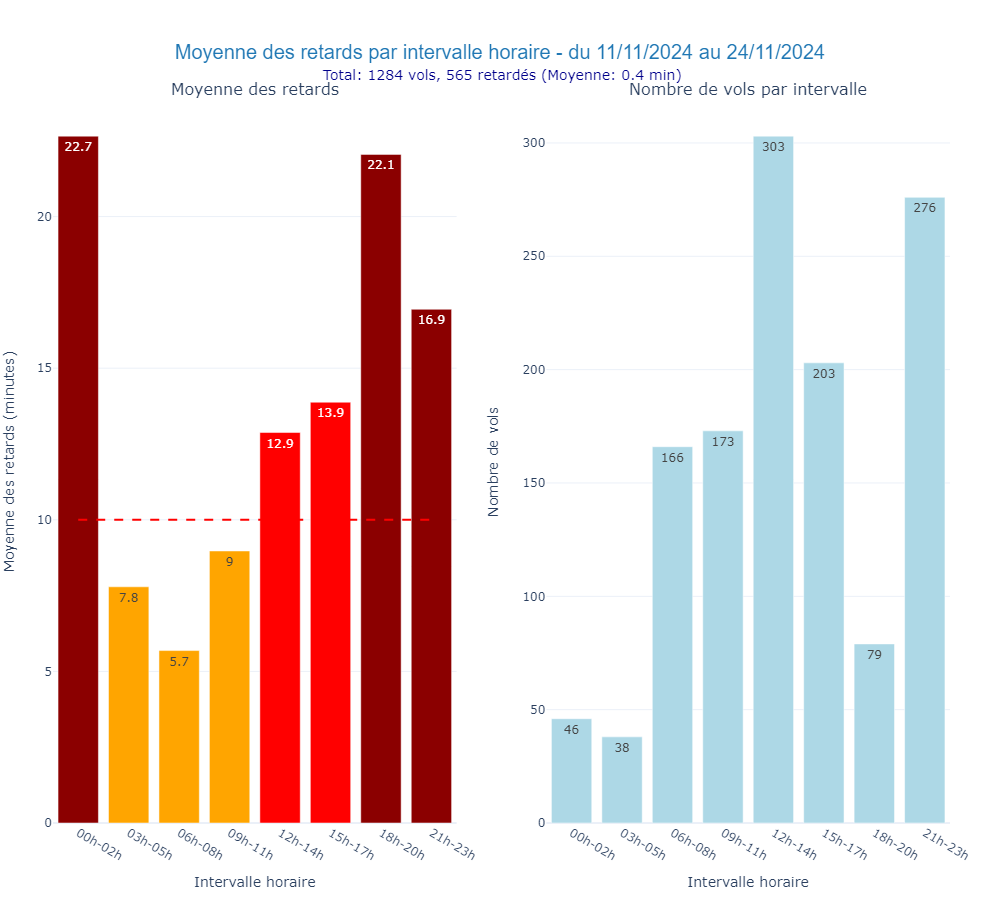
\includegraphics[width=\linewidth]{assets/dataset/parCrticite.png}
		\caption{Retard moyen par tranche horaire}
		\label{fig:retard_moyen_jour}
	\end{subfigure}
	\hfill
	\begin{subfigure}[b]{0.48\linewidth}
		\centering
		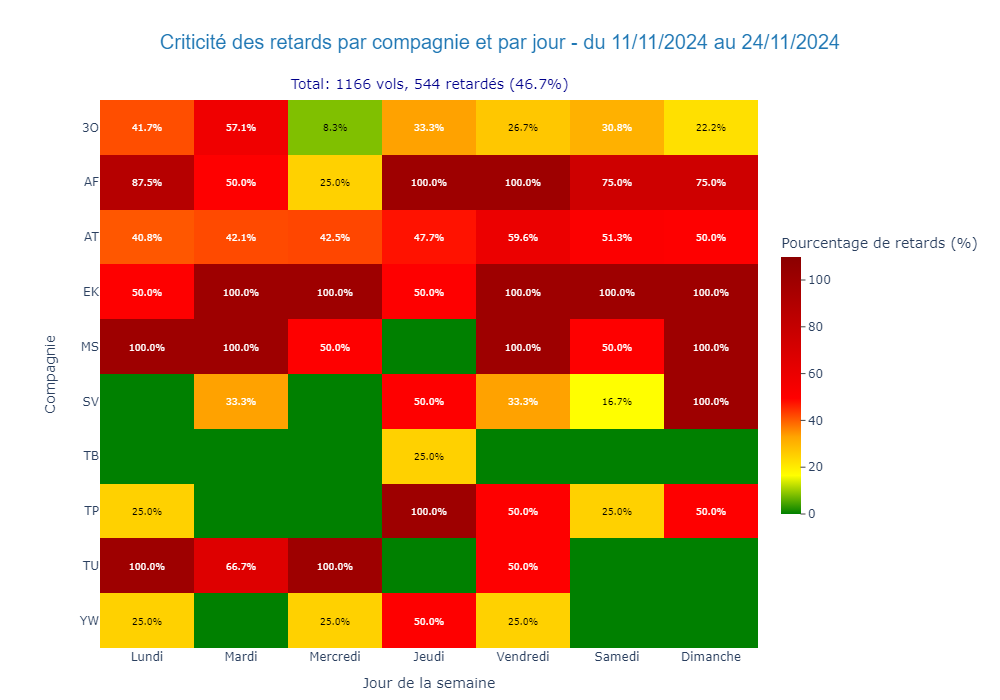
\includegraphics[width=\linewidth]{assets/dataset/parCriticite2.png}
		\caption{Retard moyen (en min) par compagnie et par jour}
		\label{fig:retard_par_heure}
	\end{subfigure}
\end{figure}

Les retards sont importants pour \textbf{TU} le lundi (135 min), ainsi que pour \textbf{AF}, \textbf{\ac{AT}}, et \textbf{MS} en milieu de semaine.  
Les pics horaires se situent entre \textbf{00h–02h} et \textbf{21h–23h} (\ref{fig:retard_par_heure}).

	
	\item \textbf{Retards selon la taille des avions}
	
	L’analyse s’appuie sur le \texttt{MTW} (poids maximal au décollage) pour estimer la taille des avions.
	
	\begin{itemize}
		\item \textbf{Small} : moins de 7 000 kg
		\item \textbf{Medium} : entre 7 000 et 136 000 kg
		\item \textbf{Large} : entre 136 000 et 250 000 kg
		\item \textbf{Super} : plus de 250 000 kg
	\end{itemize}
	 \vspace{-0.7em}
	\begin{figure}[H]
		\centering
		\begin{subfigure}[b]{0.49\linewidth}
			\centering
			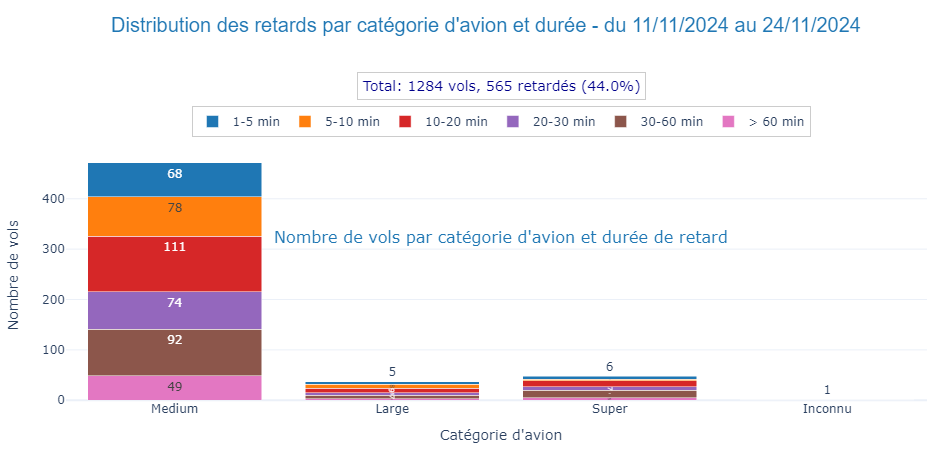
\includegraphics[width=\linewidth]{assets/dataset/tailleAvion.png}
			\caption{Retards par durée (catégorie Medium)}
			\label{fig:duree_medium}
		\end{subfigure}
		\hfill
		\begin{subfigure}[b]{0.49\linewidth}
			\centering
			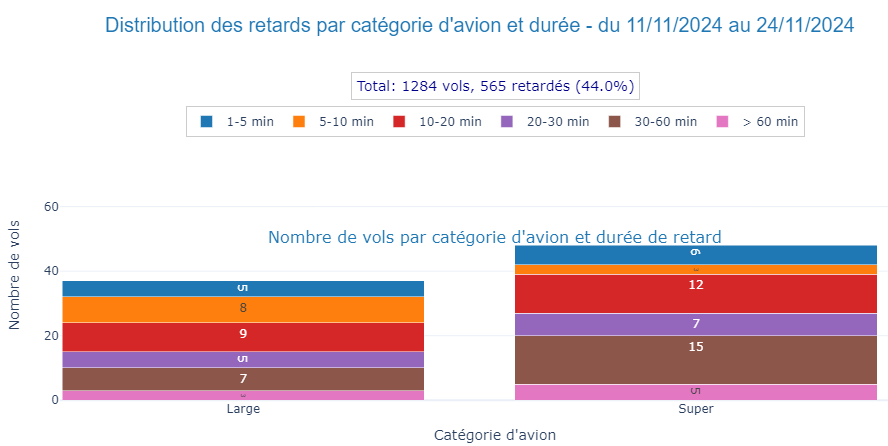
\includegraphics[width=\linewidth]{assets/dataset/tailleAvion2.png}
			\caption{Retards (hors Medium)}
			\label{fig:duree_autres}
		\end{subfigure}
	\end{figure}
	 \vspace{-0.7em}
	Les avions \textbf{Medium} concentrent 479 cas de retard. Deux pics sont notés : entre \textbf{7h–15h} (pic à 13h) et \textbf{21h–22h}.
\end{enumerate}
\vspace{-1.8em}
\section{Préparation des données}
Puisque notre dataset initial est volumineux et que les algorithmes d'affectation nécessitent une base de données optimisée.
\vspace{-1.4em}
\subsection{Fusion des datasets d’arrivée et de départ}
Nous avons opté pour la génération de deux jeux de données distincts : le dataset des vols et celui des stands. Cette génération est basée sur des recherches, notamment l'article de \cite{NilBusquetsTrias}.

Dans un premier temps, nous disposons de deux datasets initiaux : l’un relatif aux arrivées et l’autre aux départs. Chaque vol est donc représenté par une paire — un vol d’arrivée suivi d’un vol de départ, séparés par une période de stationnement. Il est ainsi essentiel de combiner correctement ces deux datasets afin de regrouper les informations d’un vol dans une seule entrée.

Pour effectuer cette fusion, nous nous sommes appuyés sur deux colonnes clés : \texttt{VID}, qui représente un identifiant unique pour chaque vol, et \texttt{REG}, correspondant à l’immatriculation de l’avion. L'utilisation conjointe de ces deux attributs nous a permis de réaliser une correspondance fiable entre les vols d’arrivée et de départ.

\subsubsection*{Les points bloquants}

Lors du processus de fusion des deux jeux de données (arrivées et départs), plusieurs incohérences et cas particuliers ont été identifiés, constituant ainsi des points bloquants :

\begin{itemize}
	\item Certaines compagnies aériennes apparaissent uniquement dans le dataset des départs (par exemple : \textbf{QS}\footnote{QS : Smartwings (République tchèque)}, \textbf{WT}\footnote{WT : Swiftair (Espagne)}), mais sont absentes du dataset des arrivées.
	\item D'autres compagnies sont présentes dans les arrivées (comme \textbf{V7}\footnote{V7 : Volotea (Espagne)}, \textbf{VY}\footnote{VY : Vueling Airlines (Espagne)}), mais ne figurent pas dans les départs.
	\item Certains vols de départ n’ont pas de correspondance dans les arrivées, ce qui rend la liaison incohérente.
	\item De même, certains vols d’arrivée ne sont liés à aucun vol de départ.
\end{itemize}


Afin de garantir l’intégrité du dataset final, nous avons choisi d’exclure ces cas lors de la fusion. Toutefois, ces anomalies soulèvent des interrogations auxquelles nous n'avons pas encore de réponse. 

\subsection{Génération du dataset des vols}

La première étape dans la création du dataset des vols consiste à sélectionner les colonnes pertinentes. Pour cela, nous avons utilisé à la fois :

\begin{itemize}
	\item des colonnes déjà présentes dans le dataset, telles que : le type d’avion, le numéro d’immatriculation, les heures d’arrivée et de départ, ainsi que le code IATA de la compagnie aérienne ;
	\item des colonnes générées à partir d’analyses préalables, notamment : \texttt{day} (le jour de la semaine), \texttt{classification\_aircraft\_size} (la taille de l’avion, classée en small, medium, large ou super), et \texttt{delay\_severity} (qui représente la sévérité du retard : faible, moyen ou élevé).
\end{itemize}

\begin{figure}[H]
	\centering
	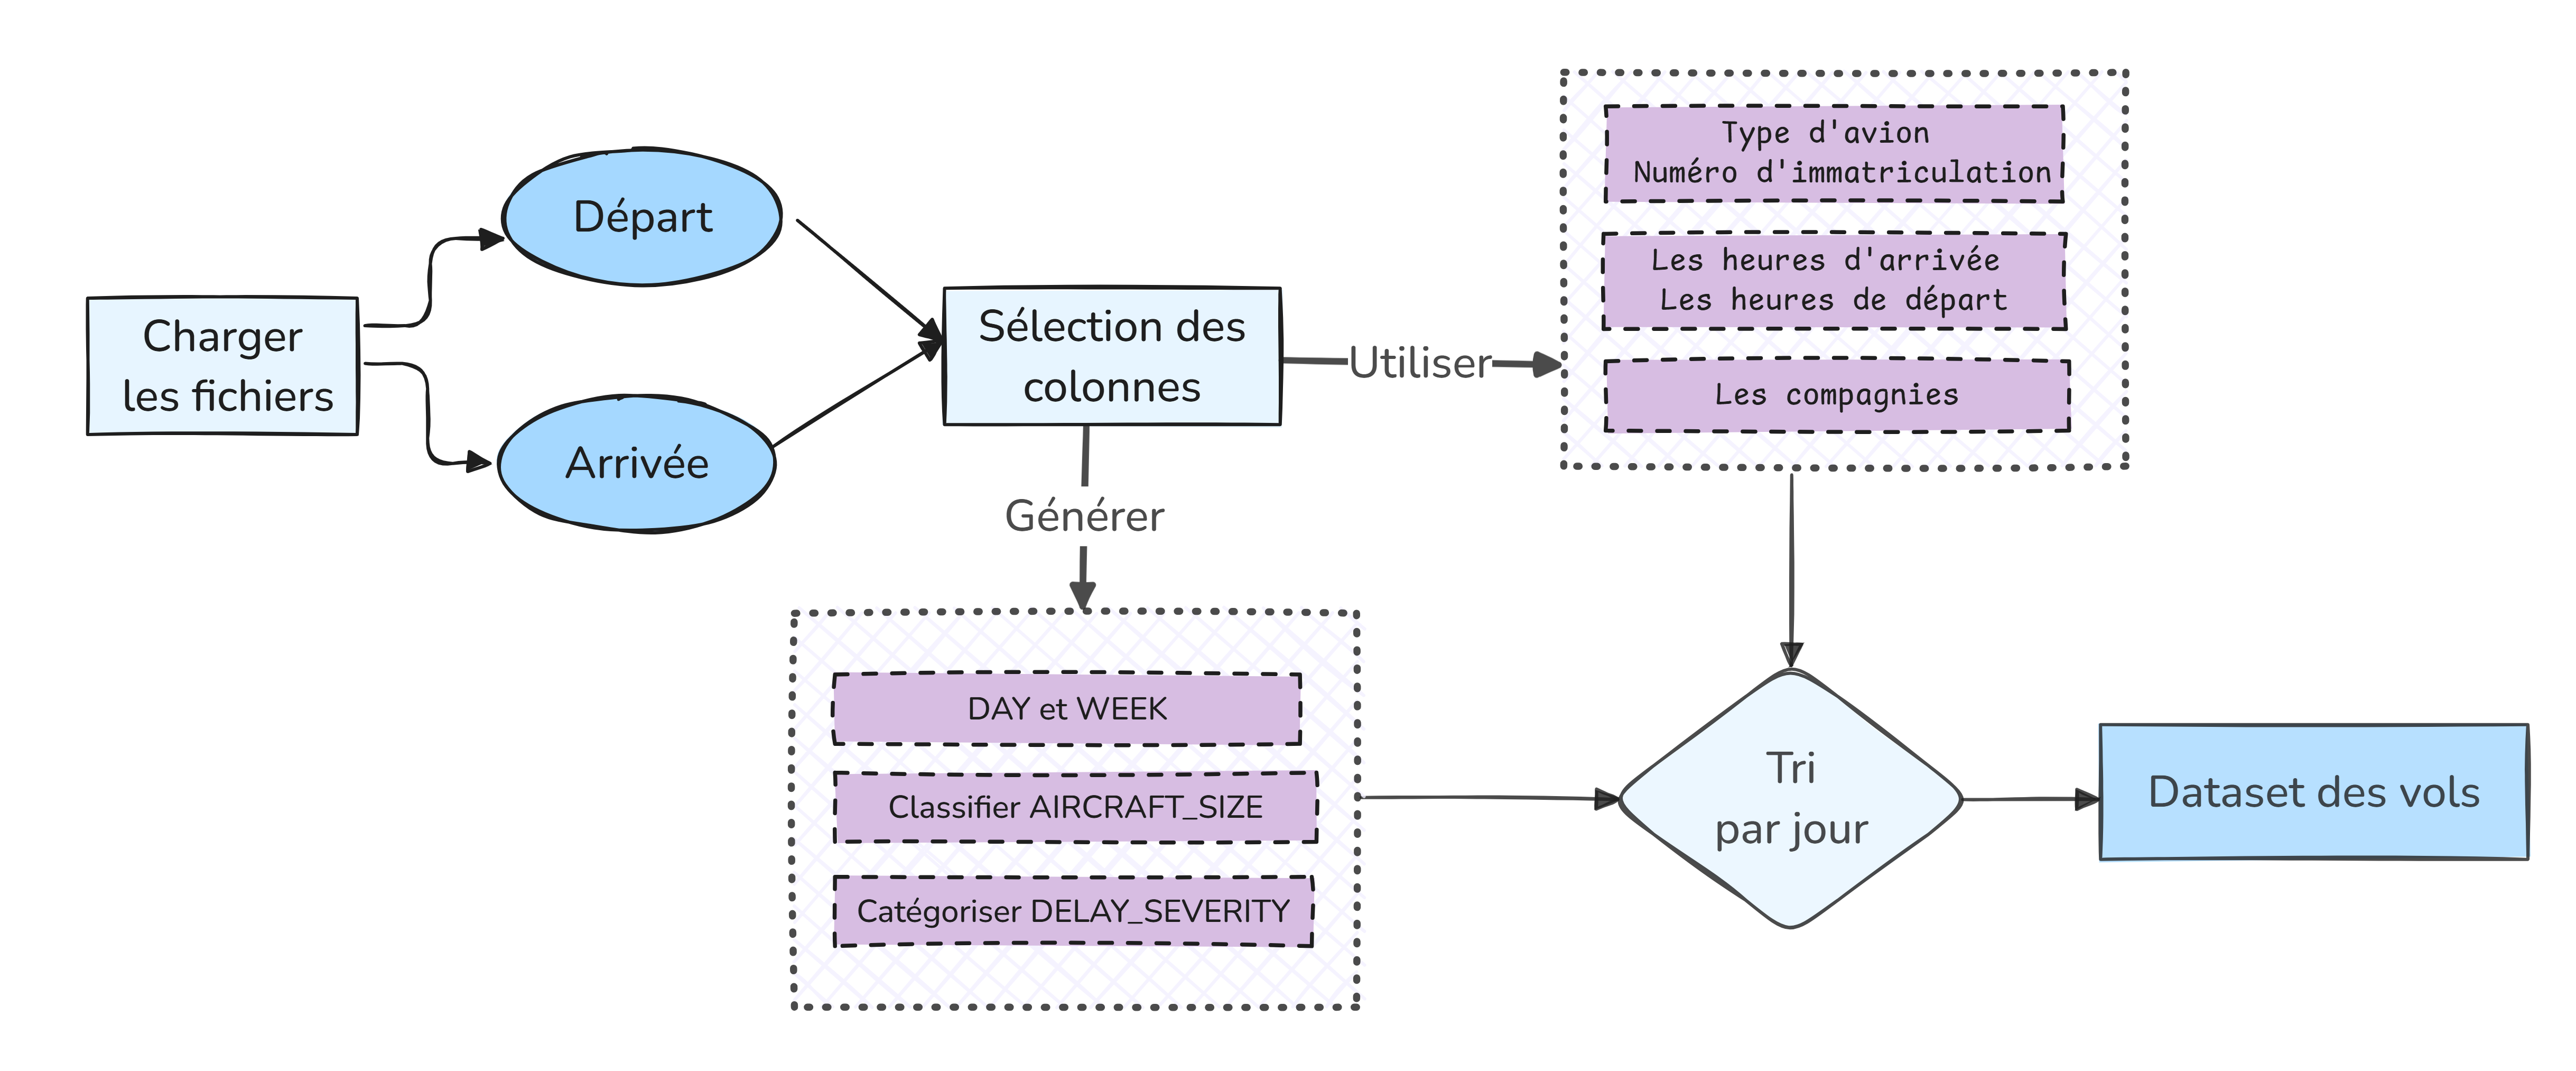
\includegraphics[width=0.9\linewidth]{assets/dataset/dataset_vol.png}
	\caption{Organigramme du processus de génération de la donnée des vols}
	\label{fig:Organigramme_vol}
\end{figure}
Le tableau suivant présente la catégorie de chaque colonne utilisée, avec le nom des colonnes, leur description et un exemple.
\begin{table}[H]
	\scriptsize
	\renewcommand{\arraystretch}{1.5}
	\caption{Jeu de données vols - Aperçu des attributs clés}
	\begin{tabularx}{\textwidth}{@{} p{3cm} p{2.7cm} X p{3.5cm} @{}}
		\toprule
		\textbf{Catégorie} & \textbf{Attribut} & \textbf{Description} & \textbf{Exemple / Type} \\
		\midrule
		
		\multirow{3}{*}{Identification du vol} & \texttt{VID} & Identifiant unique du vol & \textit{1033854621, 1033623311} \\
		\cline{2-4}
		& \texttt{FLC} & Code IATA de la compagnie aérienne & AF, LH, BA \\
		\cline{2-4}
		& \texttt{TOF} & Type de vol & Domestique, International \\
		\midrule
		
		\multirow{3}{*}{Informations avion} & \texttt{TYP} & Modèle de l’avion & A320, B737-800 \\
		\cline{2-4}
		& \texttt{REG} & Immatriculation de l’avion & FHTVS, 5CBDV \\
		\cline{2-4}
		& \texttt{SIZE} & Taille de l’avion & Petit/Moyen, Grand/Super \\
		\midrule
		
		\multirow{3}{*}{Informations temporelles} & \texttt{DAY\_DEP} & Jour du départ & Lundi, Mardi \\
		\cline{2-4}
		& \texttt{WEEK} & Numéro de semaine & 1-52 \\
		\cline{2-4}
		& \texttt{H\_DEP/H\_ARR} & Heures de départ/arrivée & 08:30, 14:15 \\
		\midrule
		
		\multirow{2}{*}{Données opérationnelles} & \texttt{SCH} & Classification zone Schengen & Oui/Non \\
		\cline{2-4}
		& \texttt{DELAY\_SEVERITY} & Classification des retards & Faible/Moyen/Élevé \\
		\bottomrule
	\end{tabularx}
	\label{tab:attributs_vols}
\end{table}




Une fois ces colonnes sélectionnées, les données ont été triées par jour. Nous avons ainsi obtenu un dataset final des vols structuré et prêt à être utilisé dans les algorithmes d’affectation.

\begin{table}[H]
	\scriptsize
	\renewcommand{\arraystretch}{0.9}
	\caption{Extrait du dataset des vols avec détails départ/arrivée et sévérité des retards}
	\begin{tabularx}{1.1\textwidth}{@{}p{1.2cm} p{1.05cm} p{1.05cm} p{0.7cm} p{0.4cm} p{0.4cm} p{0.6cm} p{0.6cm} p{0.7cm} p{0.9cm} p{0.9cm} p{0.6cm} p{1cm} p{0.6cm}@{}}
		\toprule
		\textbf{VID} & \textbf{DAY\_DEP} & \textbf{DAY\_ARR} & \textbf{WEEK} & \textbf{SCH} & \textbf{TOF} & \textbf{TYP} & \textbf{FLC} & \textbf{REG} & \textbf{SIZE} & \textbf{H\_DEP} & \textbf{D\_DEP} & \textbf{H\_ARR} & \textbf{D\_ARR} \\
		\midrule
		1033854621 & 24-11-01 & 24-11-01 & S44 & NO & I & 737 & TO & FHTVS & Medium & 08:49 & Aucun & 08:04 & Aucun \\
		
		1033623311 & 24-11-01 & 24-11-01 & S44 & NO & I & 320 & U2 & OEICJ & Medium & 09:30 & Aucun & 08:30 & Aucun \\
		
		1033654091 & 24-11-01 & 24-11-01 & S44 & Y & I & 737 & AT & CNRGF & Medium & 09:40 & Élevé & 08:36 & Aucun \\
		
		1033916281 & 24-11-01 & 24-11-01 & S44 & NO & I & 320 & U2 & OEING & Medium & 10:30 & Faible & 09:30 & Aucun \\
		
		1034969151 & 24-11-01 & 24-11-01 & S44 & NO & I & 320 & U2 & GUZHU & Medium & 14:20 & Aucun & 11:20 & Aucun \\
		
		1035003971 & 24-11-01 & 24-11-01 & S44 & NO & I & 320 & WK & HBIJV & Medium & 14:25 & Aucun & 11:30 & Moyen \\
		\bottomrule
	\end{tabularx}
	\label{tab:extrait-vols}
\end{table}




\subsection{Génération du dataset des stands}

Le processus de génération du jeu de données des \textbf{stands} repose sur une série d'étapes de traitement, de nettoyage et d’enrichissement à partir des mouvements d’aéronefs enregistrés sur la plateforme aéroportuaire. Le schéma ci-dessous illustre globalement cette chaîne de traitement.

\begin{figure}[H]
	\centering
	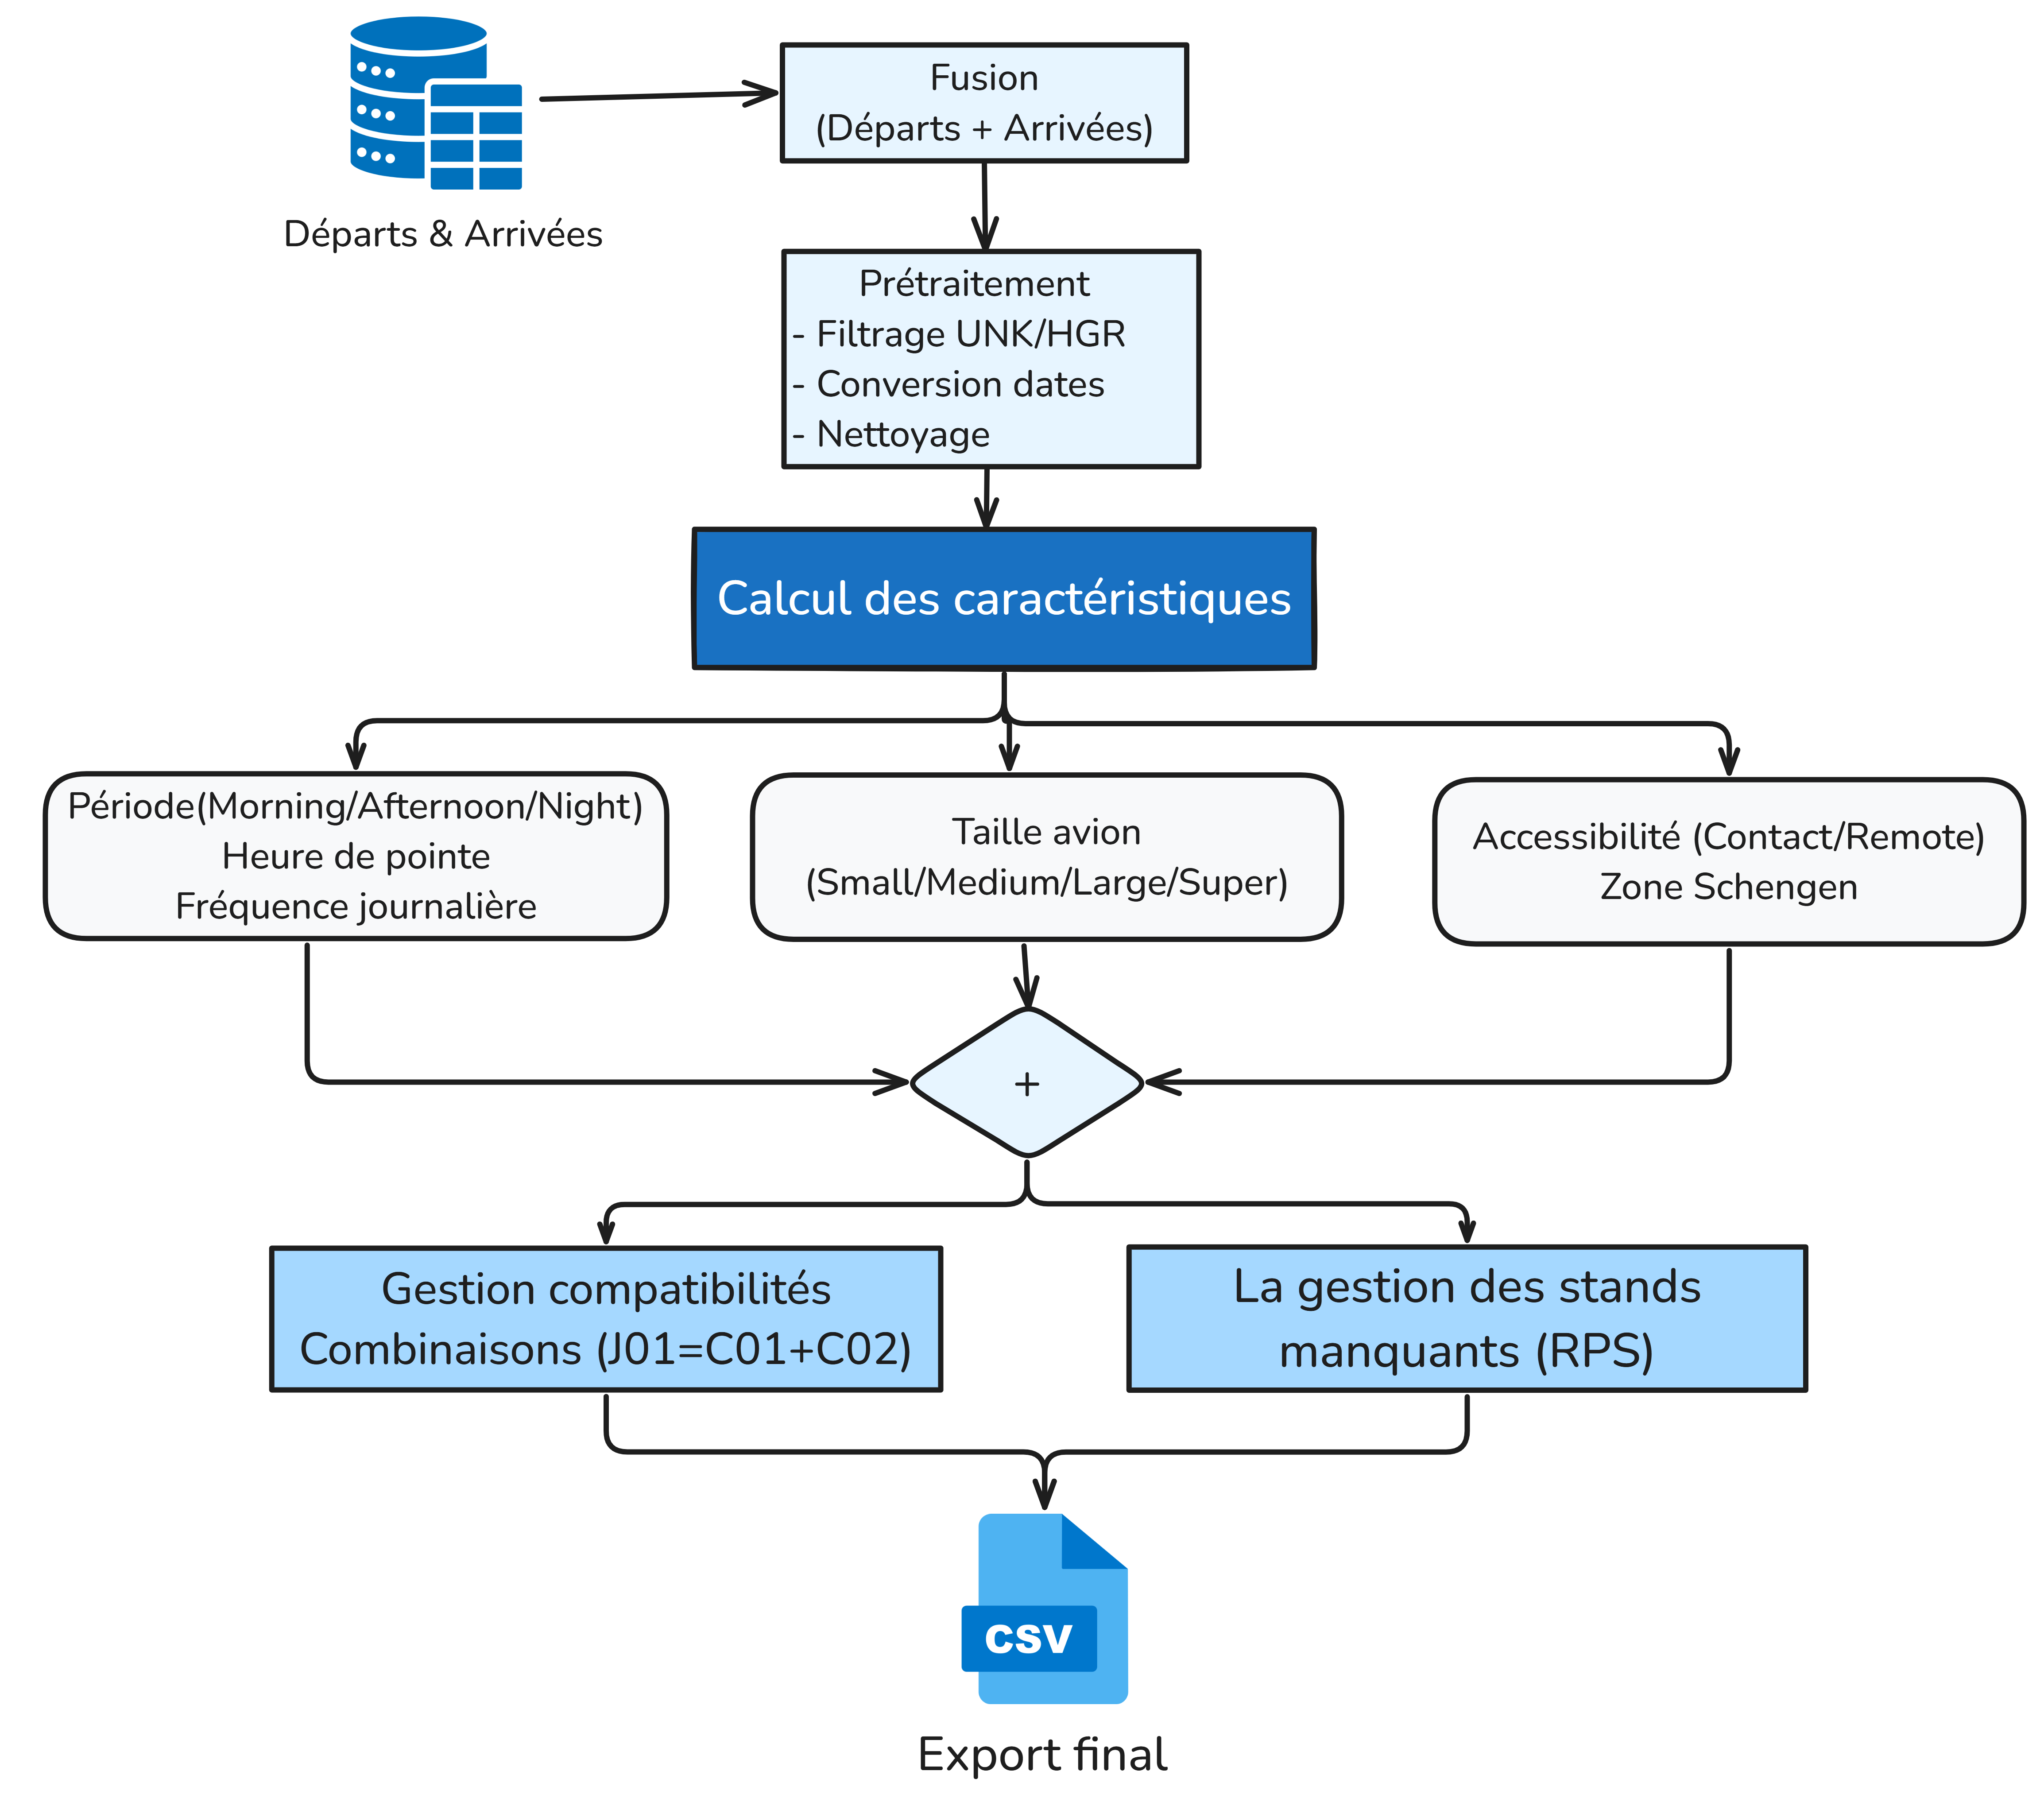
\includegraphics[width=0.6\textwidth]{assets/dataset/stand_generation.png}
	\caption{Organigramme du processus de génération de la donnée des stands}
	\label{fig:process-stands}
\end{figure}

Le traitement des données des stands s'est déroulé comme suit :

\begin{enumerate}
	\item \textbf{Collecte des données opérationnelles} à partir des historiques de mouvements d'aéronefs, en incluant :
	\begin{itemize}
		\item Le stand utilisé (\texttt{TAR}),
		\item La position de remorquage associée (\texttt{RPS}),
		\item La masse maximale au décollage (\texttt{MTW}),
		\item Le type et sous-type de l’aéronef (\texttt{TYP}, \texttt{TYS}).
	\end{itemize}
	
	\item \textbf{Nettoyage des données} :
	\begin{itemize}
		\item Suppression des enregistrements comportant des types d’aéronefs inconnus,
		\item Exclusion des aéronefs stationnés dans des hangars (\texttt{RPS = HGR}).
	\end{itemize}
	
	\item \textbf{Harmonisation et enrichissement temporel} :
	\begin{itemize}
		\item Conversion des horaires en heure locale,
		\item Déduction de la période de la journée (matin, après-midi, nuit),
		\item Identification de l’heure de pointe d’utilisation du stand (la plus fréquente),
		\item Calcul et normalisation de la fréquence maximale d’occupation journalière.
	\end{itemize}
	
	\item \textbf{Agrégation par stand} (\texttt{TAR}) afin de résumer les informations :
	\begin{itemize}
		\item Compagnies aériennes opérantes (\texttt{FLC}),
		\item Types et sous-types d'avions (\texttt{TYP}, \texttt{TYS}),
		\item Présence d’une passerelle d’embarquement (\texttt{PBB}),
		\item Statut Schengen (\texttt{SCH}).
	\end{itemize}
	
	\item \textbf{Gestion des stands non référencés} :
	\begin{itemize}
		\item Les stands uniquement présents dans \texttt{RPS} ont été considérés comme dépendants,
		\item Leurs caractéristiques ont été héritées des stands correspondants.
	\end{itemize}
	
	\item \textbf{Ajout d’une colonne de compatibilité} :
	\begin{itemize}
		\item Pour modéliser les relations fonctionnelles entre les stands,
		\item Exemple : \texttt{J01} compatible avec \texttt{C01} et \texttt{C02} (Voir Annexe \ref{fig:plan}).
	\end{itemize}
\end{enumerate}

Ce dataset consolidé fournit une base de connaissance robuste et à haute valeur ajoutée, prête à être exploitée par des algorithmes de prédiction, d’optimisation ou d’aide à la décision pour une meilleure gestion des ressources au sol dans l’environnement aéroportuaire.


\begin{table}[H]
	\centering
	\renewcommand{\arraystretch}{0.85}
	\caption{Extrait représentatif des données des stands après traitement}
	\begin{tabular}{l l l l l l l}
		\toprule
		\textbf{Stand} & \textbf{SCH} & \textbf{Fréquence} & \textbf{Heure de pointe} & \textbf{Taille Max} & \textbf{Accès} & \textbf{Compatibilité} \\
		\midrule
		B01 & YES & 21 & 10:00 PM & Medium & Contact & B01, J05, J05 \\
		\midrule
		B04 & NO  & 20 & 02:00 PM  & Medium & Contact & B04, J06, J06 \\
		\midrule
		E05 & YES & 12 & 12:00 AM  & Medium & Remote &  \\
		\midrule
		J06 & NO & 18 & 08:00 AM  & Super & Contact & J06, B03, B04 \\
		\midrule
		C23 & YES & 6 & 07:00 AM  & Super & Remote & \\
		\midrule
		B02 & NO  & 6  & 10:00 PM & Medium & Contact & B02, J05, J05 \\
		\bottomrule
	\end{tabular}
	\label{tab:extrait-stands}
\end{table}
Au total, le dataset des stands généré contient \textbf{63 lignes}, chacune représentant un stand unique, et \textbf{6 variables} principales : 
\textbf{SCH} (planification Schengen), \textbf{Fréquence} d’occupation quotidienne, \textbf{Heure de pointe}, \textbf{Taille maximale} du stand (selon la masse maximale des aéronefs accueillis), \textbf{Accès} (présence ou non de passerelle), et \textbf{Compatibilité} avec d’autres stands.
\section{Conclusion}
Dans ce chapitre, nous avons détaillé les différentes sources de données exploitées, en présentant leur structure, les variables essentielles, ainsi que les étapes de nettoyage et de préparation. L’analyse exploratoire a permis d’identifier les particularités du trafic aérien et de l’utilisation des ressources aéroportuaires.

Le chapitre suivant sera consacré à la modélisation mathématique du problème d’affectation des vols aux stands, en s’appuyant sur une revue des approches existantes, une formulation multi-objectifs et une présentation des algorithmes d’optimisation retenus.
